\chapter{Lie Algebras}

\section{DEFINITION OF LIE ALGEBRAS}

\subsection{ALGEBRAS}

Let \(\mathbf{M}\) be a unitary module over \(\mathbf{K}\) with a bilinear mapping \((x,y)\mapsto xy\) of \(\mathbf{M}\times \mathbf{M}\) into \(\mathbf{M}\) . All the axioms for algebras are satisfied except associativity of multiplication. By an abuse of language, \(\mathbf{M}\) is called a not necessarily associative algebra over \(\mathbf{K}\) , or sometimes, when no confusion can arise, an algebra over \(\mathbf{K}\) . In this no. we shall use the latter notation.

If the K-module M is given the multiplication \((x,y)\mapsto yx\) an algebra is obtained called the opposite of the above algebra.

A sub-K-module N of M which is stable under multiplication is given the structure of an algebra over K in an obvious way. N is called a subalgebra of M. N is called a left (resp. right) ideal of M if the conditions \(x \in N\) , \(y \in M\) imply \(yx \in N\) (resp. \(xy \in N\) ). If N is both a left ideal and a right ideal of M, N is called a two-sided ideal of M. In this case the multiplication on M enables us to define, on passing to the quotient, a bilinear multiplication on the quotient module M/N such that M/N has an algebra structure. M/N is called the quotient algebra of M by N.

Let \(\mathbf{M}_1\) and \(\mathbf{M}_2\) be two algebras over \(\mathbf{K}\) and \(\phi\) a mapping of \(\mathbf{M}_1\) into \(\mathbf{M}_2\) . \(\phi\) is called a homomorphism if \(\phi\) is K-linear and \(\phi(xy) = \phi(x)\phi(y)\) for \(x\in \mathbf{M}_1\) , \(y\in \mathbf{M}_1\) . The kernel \(\mathbf{N}\) of \(\phi\) is a two-sided ideal of \(\mathbf{M}_1\) and the image of \(\phi\) is a subalgebra of \(\mathbf{M}_2\) . On passing to the quotient, \(\phi\) defines an isomorphism of the algebra \(\mathbf{M}_1 / N\) onto the algebra \(\phi (\mathbf{M}_1)\) .

Let \(\mathbf{M}\) be an algebra over \(\mathbf{K}\) . A mapping \(\mathbf{D}\) of \(\mathbf{M}\) into \(\mathbf{M}\) is called a derivation of \(\mathbf{M}\) if it is \(\mathbf{K}\) -linear and \(\mathrm{D}(xy) = (\mathrm{D}x)y + x(\mathrm{D}y)\) for all \(x \in \mathbf{M}\) and \(y \in \mathbf{M}\) . This definition generalizes Definition 3 of Algebra, Chapter IV, § 4, no. 3. The kernel of a derivation of \(\mathbf{M}\) is a subalgebra of \(\mathbf{M}\) . If \(\mathrm{D}_1\) and \(\mathrm{D}_2\) are derivations of \(\mathbf{M}\) , then \(\mathrm{D}_1\mathrm{D}_2 - \mathrm{D}_2\mathrm{D}_1\) is a derivation of \(\mathbf{M}\) (cf.~Algebra, Chapter IV, § 4, no. 3, Proposition 5: the proof of this proposition does not use the associativity of the algebra).

Let \(\mathbf{M}_1\) and \(\mathbf{M}_2\) be two algebras over K. On the product K-module \(\mathbf{M} = \mathbf{M}_1 \times \mathbf{M}_2\) we define a multiplication by writing

\[
(x _ {1}, x _ {2}) (y _ {1}, y _ {2}) = (x _ {1} y _ {1}, x _ {2} y _ {2}),
\]

for all \(x_1, y_1\) in \(\mathbf{M}_1, x_2, y_2\) in \(\mathbf{M}_2\) . The algebra thus defined is called the product algebra of \(\mathbf{M}_1\) and \(\mathbf{M}_2\) . The mapping \(x_1 \mapsto (x_1, 0)\) (resp. \(x_2 \mapsto (0, x_2)\) ) is an isomorphism of \(\mathbf{M}_1\) (resp. \(\mathbf{M}_2\) ) onto a two-sided ideal of M. Under these isomorphisms \(\mathbf{M}_1\) and \(\mathbf{M}_2\) are identified with two-sided ideals of M. The K-module M is then the direct sum of \(\mathbf{M}_1\) and \(\mathbf{M}_2\) . Conversely, let M be an algebra over K and \(\mathbf{M}_1, \mathbf{M}_2\) two two-sided ideals of M such that M is the direct sum of \(\mathbf{M}_1\) and \(\mathbf{M}_2\) . Then \(\mathbf{M}_1\mathbf{M}_2 \subset \mathbf{M}_1 \cap \mathbf{M}_2 = \{0\}\) ; then, if \(x_1, y_1\) belong to \(\mathbf{M}_1\) and \(x_2, y_2\) to \(\mathbf{M}_2\) , then \((x_1 + x_2)(y_1 + y_2) = x_1y_1 + x_2y_2\) , so that M is identified with the product algebra \(\mathbf{M}_1 \times \mathbf{M}_2\) . Every left (resp. right, two-sided) ideal of \(\mathbf{M}_1\) is a left (resp. right, two-sided) ideal of M. We leave to the reader the task of formulating the analogous results in the case of an arbitrary finite family of algebras.

Let \(\mathbf{M}\) be an algebra over \(\mathbf{K}\) and suppose that the \(\mathbf{K}\) -module \(\mathbf{M}\) admits a basis \((a_{\lambda})_{\lambda \in \mathbf{L}}\) . There exists a unique system \((\gamma_{\lambda \mu \nu})_{(\lambda, \mu, \nu) \in \mathbf{L} \times \mathbf{L} \times \mathbf{L}}\) of elements of \(\mathbf{K}\) such that \(a_{\lambda}a_{\mu} = \sum_{\nu} \gamma_{\lambda \mu \nu}a_{\nu}\) for all \(\lambda, \mu\) in \(\mathbf{L}\) . The \(\gamma_{\lambda \mu \nu}\) are called the constants of structure of \(\mathbf{M}\) with respect to the basis \((a_{\lambda})\) .

Let \(\mathbf{M}\) be an algebra over \(\mathbf{K}\) , \(\mathbf{K}_0\) a commutative ring with unit element and \(\rho\) a homomorphism of \(\mathbf{K}_0\) into \(\mathbf{K}\) mapping unit element to unit element. Then \(\mathbf{M}\) can be considered as an algebra over \(\mathbf{K}_0\) by writing \(\alpha.x = \rho(\alpha).x\) for \(\alpha \in \mathbf{K}_0, x \in \mathbf{M}\) . This is the case in particular when \(\mathbf{K}_0\) is a subring of \(\mathbf{K}\) containing the unit element and \(\rho\) is taken to be the inclusion mapping of \(\mathbf{K}_0\) into \(\mathbf{K}\) .

Let M be an algebra over K, \(K_{1}\) a commutative ring with unit element and \(\sigma\) a homomorphism of K into \(K_{1}\) mapping unit element to unit element. Let \(M_{(K_{1},\sigma)} = M_{(K_{1})}\) be the \(K_{1}\) -module derived from M by extending the ring of scalars to \(\mathbf{K}_1\) (Algebra, Chapter II, § 5). The product on M defines canonically a \(\mathbf{K}_1\) -bilinear mapping of \(\mathrm{M}_{(\mathbf{K}_1)} \times \mathrm{M}_{(\mathbf{K}_1)}\) into \(\mathrm{M}_{(\mathbf{K}_1)}\) (Algebra, Chapter IX, § 1, no. 4) such that \(\mathrm{M}_{(\mathbf{K}_1)}\) is given the structure of an algebra over \(\mathbf{K}_1\) (which is said to be derived from M by extending the ring of scalars to \(\mathbf{K}_1\) ). This is the case in particular when K is a subring of \(\mathbf{K}_1\) containing the unit element and \(\sigma\) the inclusion mapping of K into \(\mathbf{K}_1\) .

\subsection{LIE ALGEBRAS}

DEFINITION 1. An algebra g over K is called a Lie algebra over K if its multiplication (denoted by \((x,y)\mapsto [x,y])\) satisfies the identities:

\[
[ x, x ] = 0\tag{1}
\]

\[
[ x, [ y, z ] ] + [ y, [ z, x ] ] + [ z, [ x, y ] ] = 0\tag{2}
\]

for all x, y, z in g.

The product \([x, y]\) is called the bracket of \(x\) and \(y\) . Identity (2) is called the Jacobi identity.

The bracket \([x, y]\) is an alternating bilinear function of \(x\) and \(y\) . We have the identity:

\[
[ x, y ] = - [ y, x ]\tag{3}
\]

so that the Jacobi identity can be written:

\[
[ x, [ y, z ] ] = [ [ x, y ], z ] + [ y, [ x, z ] ].\tag{4}
\]

Every subalgebra and every quotient algebra of a Lie algebra is a Lie algebra. Every product of Lie algebras is a Lie algebra. If g is a Lie algebra, the opposite algebra \(g^{0}\) is a Lie algebra and the mapping \(x \mapsto -x\) an isomorphism of g onto \(g^{0}\) , by virtue of identity (3).

Example 1. Let L be an associative algebra over K. The bracket \([x, y] = xy - yx\) is a bilinear function of \(x\) and \(y\) . It is easily verified that the law of composition \((x, y) \mapsto [x, y]\) on the K-module L makes L into a Lie algebra over K.

Example 2. In Example 1 choose L to be the associative algebra of endomorphisms of a K-module E. We obtain the Lie algebra of endomorphisms of E, denoted by \(\mathfrak{gl}(\mathbf{E})\) . (If \(\mathbf{E} = \mathbf{K}^n\) , the Lie algebra \(\mathfrak{gl}(\mathbf{E})\) is denoted by \(\mathfrak{gl}(n, \mathbf{K})\) .)

Every Lie subalgebra of \(\mathfrak{gl}(\mathbf{E})\) is a Lie algebra over K. In particular:

\begin{enumerate}
\def\labelenumi{(\arabic{enumi})}
\item
  If E is given a (not necessarily associative) algebra structure, the derivations of E form a Lie algebra over K.
\item
  If E admits a finite basis, the endomorphisms of E of zero trace form a Lie algebra over K denoted by \(\mathfrak{sl}(\mathbf{E})\) (or \(\mathfrak{sl}(n,\mathbf{K})\) if \(E = K^{n}\) ).
\item
  The set \(\mathbf{M}_n(\mathbf{K})\) of square matrices of order \(n\) can be considered as a Lie algebra over K canonically isomorphic to \(\mathfrak{gl}(n, \mathbf{K})\) . Let \((E_{ij})\) be the canonical basis of \(\mathbf{M}_n(\mathbf{K})\) (Algebra, Chapter II, § 10, no. 3). It follows easily that:
\end{enumerate}

\[
\left\{ \begin{array}{l l} [ E _ {i j}, E _ {k l} ] = 0 & \text {if} j \neq k \quad \text {and} \quad i \neq l \\ {} [ E _ {i j}, E _ {j l} ] = E _ {i l} & \text {if} i \neq l \\ {} [ E _ {i j}, E _ {k i} ] = - E _ {k j} & \text {if} j \neq k \\ {} [ E _ {i j}, E _ {j i} ] = E _ {i i} - E _ {j j} \end{array} \right.\tag{5}
\]

The Lie subalgebra of \(\mathbf{M}_{n}(\mathbf{K})\) consisting of the triangular matrices (resp. triangular matrices of zero trace, resp. triangular matrices of zero diagonal) is denoted by \(t(n,\mathbf{K})\) (resp. \(\mathfrak{st}(n,\mathbf{K})\) , resp. \(\mathfrak{n}(n,\mathbf{K})\) ) (Algebra, Chapter II, § 10, no. 7).

*Example 3. Let V be an infinitely differentiable real manifold. The differential operators with infinitely differentiable real coefficients constitute an associative algebra over R and hence, by Example 1, a Lie algebra \(\Delta\) over R. The bracket of two infinitely differentiable vector fields on V is an infinitely differentiable vector field and hence the infinitely differentiable vector fields on V constitute a Lie subalgebra \(\mathfrak{f}\) of \(\Delta\) . If V is a real Lie group, the left invariant vector fields constitute a Lie subalgebra \(\mathfrak{g}\) of \(\mathfrak{f}\) called the Lie algebra of V. The vector space \(\mathfrak{g}\) is identified with the tangent space to V at \(e\) (the identity element of V). Let V' be another real Lie group, \(e'\) its identity element and \(\mathfrak{g}'\) its Lie algebra. Every analytic homomorphism of V into V' defines a linear mapping of the tangent space to V at \(e\) into the tangent space to V' at \(e'\) ; this mapping is a homomorphism of the Lie algebra \(\mathfrak{g}\) into the Lie algebra \(\mathfrak{g}'\) . If V is the linear group of a finite-dimensional real vector space E there exists a canonical isomorphism of gl(E) onto the Lie algebra \(\mathfrak{g}\) of V, under which \(\mathfrak{g}\) is identified with gl(E) \(_*\) .

DEFINITION 2. Let g be a Lie algebra and x an element of g. The linear mapping \(y \mapsto [x, y]\) of g into g is called the adjoint linear mapping of x and is denoted by \(ad_{g}x\) or ad x.

PROPOSITION 1. Let \(\mathfrak{g}\) be a Lie algebra. For all \(x \in \mathfrak{g}\) , ad \(x\) is a derivation. The mapping \(x \mapsto \operatorname{ad} x\) is a homomorphism of the Lie algebra \(\mathfrak{g}\) into the Lie algebra \(\mathfrak{d}\) of derivations of \(\mathfrak{g}\) . If \(\mathrm{D} \in \mathfrak{d}\) and \(x \in \mathfrak{g}\) , {[}D, ad \(x\) {]} = \(\operatorname{ad}(\mathrm{D}x)\) .

Identity (4) can be written:

\[
(\operatorname{ad} x). [ y, z ] = [ (\operatorname{ad} x). y, z ] + [ y, (\operatorname{ad} x). z ]
\]

or:

\[
(\operatorname{ad} [ x, y ]). z = (\operatorname{ad} x). ((\operatorname{ad} y). z) - (\operatorname{ad} y). ((\operatorname{ad} x). z)
\]

whence the first two assertions. On the other hand, if \(\mathbf{D} \in \mathfrak{d}\) , \(x \in \mathfrak{g}\) , \(y \in \mathfrak{g}\) , then \([\mathbf{D}, \operatorname{ad} x] \cdot y = \mathrm{D}([x, y]) - [x, \mathrm{D}y] = [\mathrm{D}x, y] = (\operatorname{ad} \mathrm{D}x) \cdot y\) , whence the last assertion.

The mapping ad \(x\) is also called the inner derivation defined by \(x\) .

\subsection{COMMUTATIVE LIE ALGEBRAS}

DEFINITION 3. Two elements \(x, y\) of a Lie algebra are said to be permutable if \([x, y] = 0\) . \(g\) is said to be commutative if any two of its elements are permutable.

Example 1. Let L be an associative algebra and g the Lie algebra defined by it (no. 2, Example 1). Two elements x, y are permutable in g if and only if xy = yx in L.

*Example 2. If a real Lie group G is commutative, its Lie algebra is commutative.*

Every K-module can obviously be given a unique commutative Lie algebra structure over K.

If g is a Lie algebra, every monogenous submodule of g is a commutative Lie subalgebra of g.

\subsection{IDEALS}

It follows from identity (3) that in a Lie algebra \(\mathfrak{g}\) there is no distinction between left ideals and right ideals, every ideal being two-sided. We therefore speak simply of ideals.

*Example. Let G be a Lie group, g its Lie algebra and H a Lie subgroup of G. Every left invariant vector field on H defines canonically a left invariant vector field on G, whence there is a canonical injection of the Lie algebra h of H into g; h is identified with a Lie subalgebra of g under this injection. If H is normal in G, the canonical image of h in g is an ideal of g.*

An ideal of g is a submodule of g which is stable under the inner derivations of g.

DEFINITION 4. A submodule of g which is stable under every derivation of g is called a characteristic ideal of g.

PROPOSITION 2. Let g be a Lie algebra, a an ideal (resp. a characteristic ideal) of g and b a characteristic ideal of a. Then b is an ideal (resp. a characteristic ideal) of g.

Every inner derivation (resp. every derivation) of g leaves a stable and induces on a a derivation and hence leaves b stable.

Let \(\mathfrak{g}\) be a Lie algebra. If \(\mathfrak{a}\) and \(\mathfrak{b}\) are ideals of \(\mathfrak{g}\) , \(\mathfrak{a} + \mathfrak{b}\) and \(\mathfrak{a} \cap \mathfrak{b}\) are ideals of \(\mathfrak{g}\) .

Let \(\mathfrak{a}\) and \(\mathfrak{b}\) be two submodules of \(\mathfrak{g}\) . By an abuse of notation, the submodule of \(\mathfrak{g}\) generated by the elements of the form \([x,y](x\in\mathfrak{a},y\in\mathfrak{b})\) is denoted by \([\mathfrak{a},\mathfrak{b}]\) . We have \([\mathfrak{a},\mathfrak{b}] = [\mathfrak{b},\mathfrak{a}]\) by identity (3). If \(z\in\mathfrak{g}\) , \([z,\mathfrak{a}]\) , or \([\mathfrak{a},z]\) , denotes the submodule \([\mathrm{K}z,\mathfrak{a}] = (\mathrm{ad}\,z)(\mathfrak{a})\) .

PROPOSITION 3. If a and b are ideals (resp. characteristic ideals) of g, {[}a, b{]} is an ideal (resp. a characteristic ideal) of g.

Let D be an inner derivation (resp. a derivation) of g. If \(x \in a\) and \(y \in b\) , then

\[
\mathrm{D} ([ x, y ]) = [ \mathrm{D} x, y ] + [ x, \mathrm{D} y ] \in [ \mathfrak {a}, \mathfrak {b} ].
\]

Hence the proposition.

If \(\mathfrak{a}\) is a submodule of \(\mathfrak{g}\) , the set of \(x \in \mathfrak{g}\) such that (ad \(x\) ). \(\mathfrak{a} \subset \mathfrak{a}\) is a subalgebra \(\mathfrak{n}\) of \(\mathfrak{g}\) called the normalizer of \(\mathfrak{a}\) in \(\mathfrak{g}\) . If further \(\mathfrak{a}\) is a subalgebra of \(\mathfrak{g}\) , then \(\mathfrak{a} \subset \mathfrak{n}\) and \(\mathfrak{a}\) is an ideal of \(\mathfrak{n}\) .

\subsection{DERIVED SERIES, LOWER CENTRAL SERIES}

The characteristic ideal \([\mathfrak{g},\mathfrak{g}]\) is called the derived ideal of a Lie algebra \(\mathfrak{g}\) and denoted by \(\mathcal{D}\mathfrak{g}\) .

Every submodule of g containing \(\mathcal{D}\mathfrak{g}\) is an ideal of g.

The derived series of \(\mathfrak{g}\) is the decreasing sequence \(\mathcal{D}^0\mathfrak{g},\mathcal{D}^1\mathfrak{g},\ldots\) of characteristic ideals of \(\mathfrak{g}\) defined inductively as follows: (1) \(\mathcal{D}^0\mathfrak{g} = \mathfrak{g}\) ; (2) \(\mathcal{D}^{p + 1}\mathfrak{g} = [\mathcal{D}^p\mathfrak{g},\mathcal{D}^p\mathfrak{g}]\) .

The lower central series of g is the decreasing sequence \(\mathcal{C}^1\mathfrak{g},\mathcal{C}^2\mathfrak{g},\ldots\) of characteristic ideals of g defined inductively as follows: (1) \(\mathcal{C}^1\mathfrak{g} = \mathfrak{g}\) ; (2) \(\mathcal{C}^{p + 1}\mathfrak{g} = [\mathfrak{g},\mathcal{C}^p\mathfrak{g}]\) . Then \(\mathcal{C}^2\mathfrak{g} = \mathcal{D}\mathfrak{g}\) and \(\mathcal{C}^{p + 1}\mathfrak{g}\supset \mathcal{D}^{p}\mathfrak{g}\) for all \(p\) , as is immediately seen by induction on \(p\) .

PROPOSITION 4. Let \(\mathfrak{g}\) and \(\mathfrak{h}\) be two Lie algebras over \(\mathbf{K}\) and \(f\) a homomorphism of \(\mathfrak{g}\) onto \(\mathfrak{h}\) . Then \(f(\mathcal{D}^p\mathfrak{g}) = \mathcal{D}^{p}\mathfrak{h}, f(\mathcal{C}^p\mathfrak{g}) = \mathcal{C}^{p}\mathfrak{h}\) .

If a and b are submodules of g, it follows immediately that

\[
f ([ \mathfrak {a}, \mathfrak {b} ]) = [ f (\mathfrak {a}), f (\mathfrak {b}) ].
\]

The proposition is then immediate by induction on p.

COROLLARY. Let g be a Lie algebra and a an ideal of g. For the Lie algebra g/a to be commutative, it is necessary and sufficient that a ⊃ \(\mathcal{D}\mathfrak{g}\).

To say that \(\mathfrak{g} / \mathfrak{a}\) is commutative amounts to saying that \(\mathcal{D}(\mathfrak{g} / \mathfrak{a}) = \{0\}\) . But \(\mathcal{D}(\mathfrak{g} / \mathfrak{a})\) is, by Proposition 4, the canonical image of \(\mathcal{D}\mathfrak{g}\) in \(\mathfrak{g} / \mathfrak{a}\) .

\subsection{UPPER CENTRAL SERIES}

Let \(\mathfrak{g}\) be a Lie algebra and \(\mathbf{P}\) a subset of \(\mathfrak{g}\) . The centralizer of \(\mathbf{P}\) in \(\mathfrak{g}\) is the set of elements of \(\mathfrak{g}\) which are permutable with those of \(\mathbf{P}\) . This centralizer is the intersection of the kernels of the ad \(y\) , where \(y\) runs through \(\mathbf{P}\) ; it is therefore a subalgebra of \(\mathfrak{g}\) .

PROPOSITION 5. Let g be a Lie algebra and a an ideal (resp. a characteristic ideal) of g. The centralizer \(\mathfrak{a}'\) of a in g is an ideal (resp. a characteristic ideal) of g.

Let \(D\) be an inner derivation (resp. a derivation) of \(g\) . If \(x \in a'\) and \(y \in a\) , then

\[
[ \mathrm{D} x, y ] = \mathrm{D} ([ x, y ]) - [ x, \mathrm{D} y ] = 0;
\]

hence \(\mathrm{D}x\in \mathfrak{a}^{\prime}\) . Hence the proposition.

Let g be a Lie algebra. The centralizer of g in g is called the centre of g, that is the characteristic ideal of \(x \in g\) such that \([x, y] = 0\) for all \(y \in g\) . The centre of g is the kernel of the homomorphism \(x \mapsto ad x\) .

The upper central series of \(\mathfrak{g}\) is the increasing sequence \(\mathcal{C}_{0}\mathfrak{g},\mathcal{C}_{1}\mathfrak{g},\ldots\) of characteristic ideals of \(\mathfrak{g}\) defined inductively as follows: (1) \(\mathcal{C}_{0}\mathfrak{g} = \{0\}\) ; (2) \(\mathcal{C}_{p + 1}\mathfrak{g}\) is the inverse image under the canonical mapping of \(\mathfrak{g}\) onto \(\mathfrak{g} / \mathcal{C}_{p}\mathfrak{g}\) of the centre of \(\mathfrak{g} / \mathcal{C}_{p}\mathfrak{g}\) .

The ideal \(\mathcal{C}_{1}\mathfrak{g}\) is the centre of \(\mathfrak{g}\) .

\subsection{EXTENSIONS}

DEFINITION 5. Let \(\mathfrak{a}\) and \(\mathfrak{b}\) be two Lie algebras over \(\mathbf{K}\) . An extension of \(\mathfrak{b}\) by \(\mathfrak{a}\) is a sequence:

\[
a \xrightarrow {\lambda} g \xrightarrow {\mu} b
\]

where g is a Lie algebra over K, μ a surjective homomorphism of g onto b and λ an injective homomorphism of a onto the kernel of μ.

The kernel \(\mathfrak{n}\) of \(\mu\) is called the kernel of the extension. The homomorphism \(\lambda\) is an isomorphism of \(\mathfrak{a}\) onto \(\mathfrak{n}\) and the homomorphism \(\mu\) defines an isomorphism of \(\mathfrak{g} / \mathfrak{n}\) onto \(\mathfrak{b}\) when passing to the quotient.

By an abuse of language, g is also called an extension of b by a.

Two extensions:

\[
a \xrightarrow {\lambda} g \xrightarrow {\mu} b, \quad a \xrightarrow {\lambda^ {\prime}} g ^ {\prime} \xrightarrow {\mu^ {\prime}} b
\]

are said to be equivalent if there exists a homomorphism \(f\) of \(\mathfrak{g}\) into \(\mathfrak{g}'\) such that the following diagram:

\pandocbounded{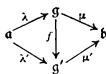
\includegraphics[keepaspectratio]{images/part001_2862d8fe.jpg}}

is commutative (that is such that \(f \circ \lambda = \lambda', \mu' \circ f = \mu\) ). We show that such a homomorphism is necessarily bijective. First \(f\) is injective. For if \(x \in \mathfrak{g}\) is such that \(f(x) = 0\) , then \(\mu(x) = \mu'(f(x)) = 0\) and hence \(x = \lambda(y)\) for some \(y \in \mathfrak{a}\) ; then \(\lambda'(y) = f(\lambda(y)) = f(x) = 0\) , hence \(y = 0\) and hence \(x = 0\) . On the other hand, \(f\) is surjective. For \(\mu' \circ f = \mu\) is surjective and hence \(f(\mathfrak{g}) + \lambda'(\mathfrak{a}) = \mathfrak{g}'\) ; on the other hand \(f(\mathfrak{g}) \supset f(\lambda(\mathfrak{a})) = \lambda'( \mathfrak{a})\) .

It follows from this that the relation just defined between two extensions of b by a is an equivalence relation.

PROPOSITION 6. Let

\[
a \xrightarrow {\lambda} g \xrightarrow {\mu} b
\]

be an extension of b by a and n its kernel.

\begin{enumerate}
\def\labelenumi{(\alph{enumi})}
\item
  If there exists a subalgebra m of g supplementary to n in g, the restriction of μ to m is an isomorphism of m onto b. If v denotes the inverse isomorphism of this restriction, v is a homomorphism of b into g and μ ∘ v is the identity automorphism of b.
\item
  Conversely, if there exists a homomorphism \(v\) of \(\mathfrak{b}\) into \(\mathfrak{g}\) such that \(\mu \circ v\) is the identity automorphism of \(\mathfrak{b}\) , then \(v(\mathfrak{b})\) is a supplementary subalgebra of \(\mathfrak{n}\) in \(\mathfrak{g}\) .
\end{enumerate}

The assertions of (a) are immediate. On the other hand, let v be a homomorphism of b into g such that \(\mu \circ v\) is the identity automorphism of b. Then \(v(b)\) is a subalgebra of g and g is the direct sum of \(v(b)\) and \(\mu^{-1}(0) = n\) (Algebra, Chapter VIII, §1, no. 1).

DEFINITION 6. Let

\[
a \xrightarrow {\lambda} g \xrightarrow {\mu} b
\]

be an extension of \(\mathfrak{b}\) by \(\mathfrak{a}\) and \(\mathfrak{n}\) its kernel. This extension is called inessential (resp. trivial) if there exists a subalgebra (resp. an ideal) of \(\mathfrak{g}\) supplementary to \(\mathfrak{n}\) in \(\mathfrak{g}\) . This extension is called central if \(\mathfrak{n}\) is contained in the centre of \(\mathfrak{g}\) .

If the extension is trivial, let \(m\) be an ideal of \(g\) supplementary to \(n\) in \(g\) . Then (cf.~no. 1) \(g\) is canonically identified with the Lie algebra \(m \times n\) and hence with the Lie algebra \(a \times b\) . Conversely, let \(a\) and \(b\) be two Lie algebras; then \(a \times b\) is a trivial extension of \(b\) by \(a\) .

An inessential central extension is trivial. For let \(\mathfrak{g}\) be a Lie algebra, \(\mathfrak{n}\) an ideal of \(\mathfrak{g}\) contained in the centre of \(\mathfrak{g}\) and \(\mathfrak{m}\) a subalgebra of \(\mathfrak{g}\) supplementary to \(\mathfrak{n}\) in \(\mathfrak{g}\) . Then \([\mathfrak{m},\mathfrak{g}] = [\mathfrak{m},\mathfrak{m}] + [\mathfrak{m},\mathfrak{n}] = [\mathfrak{m},\mathfrak{m}] \subset \mathfrak{m}\) and hence \(\mathfrak{m}\) is an ideal of \(\mathfrak{g}\) .

\subsection{SEMI-DIRECT PRODUCTS}

Let \(\mathfrak{a}\) and \(\mathfrak{b}\) be two Lie algebras over \(\mathbf{K}\) . It is not easy to construct all the extensions of \(\mathfrak{b}\) by \(\mathfrak{a}\) . But we shall describe quite simply all the inessential extensions of \(\mathfrak{b}\) by \(\mathfrak{a}\) .

Let \(g\) be an inessential extension of \(b\) by \(a\) . We identify \(a\) with an ideal of \(g\) , \(b\) with a subalgebra of \(g\) supplementary to \(a\) and the module \(g\) with the module \(a \times b\) . For all \(b \in b\) , let \(\phi_b\) be the restriction to \(a\) of \(ad_g b\) ; this is a derivation of \(a\) and the mapping \(b \mapsto \phi_b\) is a homomorphism of \(b\) into the Lie algebra of derivations of \(a\) . On the other hand, for \(a, a'\) in \(a\) and \(b, b'\) in \(b\) , we have:

\[
\begin{array}{r l} {[ (a, b), (a ^ {\prime}, b ^ {\prime}) ]} & {= [ a + b, a ^ {\prime} + b ^ {\prime} ]} \\ & {= [ a, a ^ {\prime} ] + [ a, b ^ {\prime} ] + [ b, a ^ {\prime} ] + [ b, b ^ {\prime} ]} \\ & {= ([ a, a ^ {\prime} ] + \phi_ {b} a ^ {\prime} - \phi_ {b ^ {\prime}} a, [ b, b ^ {\prime} ]).} \end{array}\tag{6}
\]

Conversely, let \(\mathfrak{a}\) and \(\mathfrak{b}\) be Lie algebras over \(\mathbf{K}\) and \(b \mapsto \phi_b\) a homomorphism of \(\mathfrak{b}\) into the Lie algebra of derivations of \(\mathfrak{a}\) . On the product \(\mathfrak{g}\) of the K-modules \(\mathfrak{a}\) and \(\mathfrak{b}\) we define the bracket of two elements by writing:

\[
[ (a, b), (a ^ {\prime}, b ^ {\prime}) ] = ([ a, a ^ {\prime} ] + \phi_ {b} a ^ {\prime} - \phi_ {b ^ {\prime}} a, [ b, b ^ {\prime} ])
\]

for all \(a, a'\) in \(\mathfrak{a}, b, b'\) in \(\mathfrak{b}\) . It is immediate that this bracket is an alternating bilinear function of \((a, b), (a', b')\) ; we show that, given 3 elements \((a, b), (a', b'), (a'', b'')\) of \(\mathfrak{a} \times \mathfrak{b}\) :

\[
\begin{array}{r l} {[ (a, b), [ (a ^ {\prime}, b ^ {\prime}), (a ^ {\prime \prime}, b ^ {\prime \prime}) ] ] + [ (a ^ {\prime}, b ^ {\prime}), [ (a ^ {\prime \prime}, b ^ {\prime \prime}), (a, b) ] ]} & \\ {+ [ (a ^ {\prime \prime}, b ^ {\prime \prime}), [ (a, b), (a ^ {\prime}, b ^ {\prime}) ] ] = 0.} \end{array}\tag{7}
\]

As the left hand side of (7) is an alternating trilinear function of \((a, b)\) , \((a', b')\) , \((a'', b'')\) , it suffices to make the verification when this system of elements takes one of the following forms:

\[
(a, 0), (a ^ {\prime}, 0), (a ^ {\prime \prime}, 0)\tag{8}
\]

\[
(a, 0), (a ^ {\prime}, 0), (0, b ^ {\prime \prime})\tag{9}
\]

\[
(a, 0), (0, b ^ {\prime}), (0, b ^ {\prime \prime})\tag{10}
\]

\[
(0, b), (0, b ^ {\prime}), (0, b ^ {\prime \prime})\tag{11}
\]

In cases (8) and (11), relation (7) is an immediate consequence of the Jacobi identity in a and b. In case (9), we have

\[
\begin{array}{l} [ (a, 0), [ (a ^ {\prime}, 0), (0, b ^ {\prime \prime}) ] ] = [ (a, 0), (- \phi_ {b ^ {\prime \prime}} a ^ {\prime}, 0) ] = (- [ a, \phi_ {b ^ {\prime \prime}} a ^ {\prime} ], 0) \\ {} [ (a ^ {\prime}, 0), [ (0, b ^ {\prime \prime}), (a, 0) ] ] = [ (a ^ {\prime}, 0), (\phi_ {b ^ {\prime \prime}} a, 0) ] = ([ a ^ {\prime}, \phi_ {b ^ {\prime \prime}} a ], 0) \\ {} [ (0, b ^ {\prime \prime}), [ (a, 0), (a ^ {\prime}, 0) ] ] = [ (0, b ^ {\prime \prime}), ([ a, a ^ {\prime} ], 0) ] = (\phi_ {b ^ {\prime \prime}} ([ a, a ^ {\prime} ]), 0) \end{array}
\]

and relation (7) follows from the equation:

\[
\phi_ {b ^ {\prime \prime}} ([ a, a ^ {\prime} ]) = [ \phi_ {b ^ {\prime \prime}} a, a ^ {\prime} ] + [ a, \phi_ {b ^ {\prime \prime}} a ^ {\prime} ].
\]

In case (10), we have:

\[
[ (a, 0), [ (0, b ^ {\prime}), (0, b ^ {\prime \prime}) ] ] = [ (a, 0), (0, [ b ^ {\prime}, b ^ {\prime \prime} ]) ] = (- \phi_ {[ b ^ {\prime}, b ^ {\prime \prime} ]} a, 0)
\]

\[
[ (0, b ^ {\prime}), [ (0, b ^ {\prime \prime}), (a, 0) ] ] = [ (0, b ^ {\prime}), (\phi_ {b ^ {\prime \prime}} a, 0) ] = (\phi_ {b ^ {\prime}} \phi_ {b ^ {\prime \prime}} a, 0)
\]

\[
[ (0, b ^ {\prime \prime}), [ (a, 0), (0, b ^ {\prime}) ] ] = [ (0, b ^ {\prime \prime}), (- \phi_ {b ^ {\prime}} a, 0) ] = (- \phi_ {b ^ {\prime \prime}} \phi_ {b ^ {\prime}} a, 0)
\]

and relation (7) follows from the equation:

\[
\phi_ {[ b ^ {\prime}, b ^ {\prime \prime} ]} = \phi_ {b ^ {\prime}} \phi_ {b ^ {\prime \prime}} - \phi_ {b ^ {\prime \prime}} \phi_ {b ^ {\prime}}.
\]

Hence a Lie algebra structure has been defined on g. The mapping \((a, b) \mapsto b\) of g onto b is a homomorphism \(\mu\) whose kernel n is the ideal of elements of g of the form \((a, 0)\) . The mapping \(a \mapsto (a, 0)\) is an isomorphism \(\lambda\) of a onto n.~Hence:

\[
a \xrightarrow {\lambda} g \xrightarrow {\mu} b\tag{12}
\]

is an extension of b by a of kernel n, which is said to be canonically defined by a, b, \(\phi\) . The mapping \(b \mapsto (0, b)\) is an isomorphism v of b onto a subalgebra of g supplementary to n in g; hence the extension is inessential.

If \(a\) is identified with \(n\) under \(\lambda\) and \(b\) with \(v(b)\) under \(v\) , then, for \(a \in a\) and \(b \in b\) :

\[
(\mathrm{ad} b). a = [ (0, b), (a, 0) ] = (\phi_ {b} a, 0) = \phi_ {b} a.
\]

When \(\phi = 0\) , \(\mathfrak{g}\) is the product Lie algebra of \(\mathfrak{b}\) and \(\mathfrak{a}\) . In the general case, \(\mathfrak{g}\) is called the semi-direct product of \(\mathfrak{b}\) by \(\mathfrak{a}\) (corresponding to the homomorphism \(b \mapsto \phi_b\) of \(\mathfrak{b}\) into the Lie algebra of derivations of \(\mathfrak{a}\) ).

We have therefore established the following proposition:

PROPOSITION 7. Let a and b be two Lie algebras over K,

\[
a \xrightarrow {\lambda} g \xrightarrow {\mu} b
\]

an inessential extension of b by a, v an isomorphism of b onto a subalgebra of g such that \(\mu \circ v\) is the identity automorphism of b and \(\phi\) the corresponding homomorphism of b into the Lie algebra of derivations of a. Let

\[
a \xrightarrow {\lambda_ {0}} g _ {0} \xrightarrow {\mu_ {0}} b
\]

be the inessential extension of \(\mathfrak{b}\) by a canonically defined by \(\phi\) . Then the mapping \((a, b) \mapsto \lambda(a) + v(b)\) is an isomorphism \(f\) of \(\mathfrak{g}_0\) onto \(\mathfrak{g}\) and the following diagram

\pandocbounded{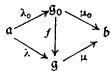
\includegraphics[keepaspectratio]{images/part001_108a7b03.jpg}}

is commutative, so that the two extensions are equivalent.

Example 1. Let g be a Lie algebra over K and D a derivation of g. Let h be the commutative Lie algebra K. The mapping \(\lambda \mapsto \lambda D (\lambda \in \mathbf{K})\) is a homomorphism of h into the Lie algebra of derivations of g. We form the corresponding semidirect product t of h by g. Let \(x_0\) be the element (0, 1) of t. For all \(x \in g\) , Dx = [x₀, x].

Example 2. Let g be a Lie algebra over K, M a K-module and \(\rho\) a homomorphism of g into gl(M). If M is considered as a commutative Lie algebra, the Lie algebra of derivations of M is gl(M). We can therefore form the semi-direct product h of g by M corresponding to \(\rho\) .

In particular, let \(\mathfrak{g} = \mathfrak{gl}(\mathbf{M})\) and \(\rho\) be the identity mapping of \(\mathfrak{gl}(\mathbf{M})\) . The semi-direct product of \(\mathfrak{g}\) by \(\mathbf{M}\) is then denoted by \(\mathfrak{af}(\mathbf{M})\) (or \(\mathfrak{af}(n,\mathbf{K})\) if \(\mathbf{M} = \mathbf{K}^{n}\) ). An element of \(\mathfrak{af}(\mathbf{M})\) is an ordered pair \((m,u)\) , where \(m\in \mathbf{M}\) , \(u\in \mathfrak{gl}(\mathbf{M})\) ; and the bracket is defined by

\[
[ (m, u), (m ^ {\prime}, u ^ {\prime}) ] = (u (m ^ {\prime}) - u ^ {\prime} (m), [ u, u ^ {\prime} ]).
\]

*When M is a finite-dimensional vector space over R, \(\mathfrak{af}(M)\) is canonically identified with the Lie algebra of the affine group of M.*

Let \(t\) be a Lie algebra over \(K\) . A linear mapping \(\theta\) of \(t\) into \(\mathfrak{af}(M)\) can be written \(x \mapsto ((\zeta(x), \eta(x))\) , where \(\zeta\) is a linear mapping of \(t\) into \(M\) and \(\eta\) a linear mapping of \(t\) into \(\mathfrak{gl}(M)\) . We examine the conditions that \(\zeta\) and \(\eta\) must satisfy for \(\theta\) to be a homomorphism. For \(x \in t, y \in t\) , we must have

\[
\theta ([ x, y ]) = [ \theta (x), \theta (y) ]
\]

that is

\[
\begin{array}{r l} (\zeta ([ x, y ]), \eta ([ x, y ])) & = [ (\zeta (x), \eta (x)), (\zeta (y), \eta (y)) ] \\ & = (\eta (x). \zeta (y) - \eta (y). \zeta (x), [ \eta (x), \eta (y) ]). \end{array}
\]

Hence for \(\theta\) to be a homomorphism of \(t\) into \(\mathfrak{af}(M)\) , it is necessary and sufficient that \(\eta\) be a homomorphism of \(t\) into \(\mathfrak{gl}(M)\) and that \(\zeta\) satisfy the relation:

\[
\zeta ([ x, y ]) = \eta (x). \zeta (y) - \eta (y). \zeta (x).\tag{13}
\]

Let \(\mathbf{N}\) be the \(\mathbf{K}\) -module \(\mathbf{M} \times \mathbf{K}\) . We take \(t\) to be the subalgebra of \(\mathfrak{gl}(\mathbf{N})\) consisting of the \(w \in \mathfrak{gl}(\mathbf{N})\) such that \(w(\mathbf{N}) \subset \mathbf{M}\) . For all \(w \in t\) , let \(\eta(w) \in \mathfrak{gl}(\mathbf{M})\) be the restriction of \(w\) to \(\mathbf{M}\) and let \(\zeta(w) = w(0,1) \in \mathbf{M}\) . For \(w_1 \in t, w_2 \in t\) ,

\[
\zeta ([ w _ {1}, w _ {2} ]) = w _ {1} (\zeta (w _ {2})) - w _ {2} (\zeta (w _ {1})) = \eta (w _ {1}). \zeta (w _ {2}) - \eta (w _ {2}). \zeta (w _ {1}).
\]

Hence the mapping \(w \mapsto (\zeta(w), \eta(w))\) is a homomorphism \(\theta\) of \(t\) into \(\mathfrak{af}(\mathbf{M})\) . Clearly \(\theta\) is bijective. Let \(\phi = \theta^{-1}\) . If \((m, u) \in \mathfrak{af}(\mathbf{M})\) , \(\phi(m, u)\) is the element \(w\) of \(t\) defined by

\[
w (m ^ {\prime}, \lambda) = (u (m ^ {\prime}) + \lambda m, 0).
\]

\(\mathfrak{af}(\mathbf{M})\) is often identified with the subalgebra \(\mathfrak{t}\) of \(\mathfrak{gl}(\mathbf{N})\) under the isomorphism \(\phi\) .

*When M is a finite-dimensional vector space over \(\mathbf{R}\) , the homomorphism \(\phi\) of \(\mathfrak{af}(M)\) into \(\mathfrak{gl}(N)\) corresponds to a canonical homomorphism \(\psi\) of the affine group A of M into the group \(\mathbf{GL}(N)\) ; if \(a \in A\) , \(\psi(a)\) is the unique element \(g\) of \(\mathbf{GL}(N)\) such that \(g(m, 1) = (a(m), 1)\) for all \(m \in M\) . This homomorphism is injective and \(\psi(A)\) is the set of automorphisms of N which leave invariant all the linear varieties of N parallel to M.*

\subsection{CHANGE OF BASE RING}

Let \(K_{0}\) be a commutative ring with unit element and \(\rho\) a homomorphism of \(K_{0}\) into K mapping unit element to unit element. Let g be a Lie algebra over K. Let \(g'\) be the algebra obtained by considering g as an algebra over \(K_{0}\) by means of \(\rho\) (cf.~no. 1). Then \(g'\) is a Lie algebra. The subalgebras (resp. ideals) of g are subalgebras (resp. ideals) of \(g'\) . If a and b are submodules of g, the bracket {[}a, b{]} is the same in g and in \(g'\) ; for {[}a, b{]} is the set of elements of the form

\(\sum_{i=1}^{n}\left[x_i,y_i\right]\) where \(x_{i}\in a,y_{i}\in b\) . It follows that \(\mathcal{D}^p\mathfrak{g} = \mathcal{D}^p\mathfrak{g}'\) , \(\mathcal{C}^p\mathfrak{g} = \mathcal{C}^p\mathfrak{g}'\) for all \(p\) .

The centralizer of a subset is the same in \(\mathfrak{g}\) and \(\mathfrak{g}'\) . Hence \(\mathcal{C}_p\mathfrak{g} = \mathcal{C}_p\mathfrak{g}'\) for all \(p\) .

Let \(\mathbf{K}_1\) be a commutative ring with unit element and \(\sigma\) a homomorphism of \(\mathbf{K}\) into \(\mathbf{K}_1\) mapping unit element to unit element. Let \(\mathfrak{g}\) be a Lie algebra over \(\mathbf{K}\) . Let \(\mathfrak{g}_{(\mathbf{K}_1)}\) be the algebra over \(\mathbf{K}_1\) derived from \(\mathfrak{g}\) by extending the base ring (cf.~no. 1). Then \(\mathfrak{g}_{(\mathbf{K}_1)}\) is a Lie algebra. If \(\mathfrak{a}\) is a subalgebra (resp. an ideal) of \(\mathfrak{g}\) , the canonical image of \(\mathfrak{a}_{(\mathbf{K}_1)}\) in \(\mathfrak{g}_{(\mathbf{K}_1)}\) is a subalgebra (resp. an ideal) of \(\mathfrak{g}_{(\mathbf{K}_1)}\) . If \(\mathfrak{a}\) and \(\mathfrak{b}\) are submodules of \(\mathfrak{g}\) , the canonical image in \(\mathfrak{g}_{(\mathbf{K}_1)}\) of \([\mathfrak{a},\mathfrak{b}]_{(\mathbf{K}_1)}\) is equal to the bracket of the canonical images of \(\mathfrak{a}_{(\mathbf{K}_1)}\) and \(\mathfrak{b}_{(\mathbf{K}_1)}\) . It follows that \(\mathcal{D}^p (\mathfrak{g}_{(\mathbf{K}_1)})\) is the canonical image of \((\mathcal{D}^p\mathfrak{g})_{(\mathbf{K}_1)}\) and that \(\mathcal{C}^p (\mathfrak{g}_{(\mathbf{K}_1)})\) is the canonical image of \((\mathcal{C}^p\mathfrak{g})_{(\mathbf{K}_1)}\) .

If K is a field, \(K_{1}\) an extension field of K and \(\sigma\) the canonical injection of K into \(K_{1}\) , then with the usual identifications we have

\[
\begin{array}{c} [ a, b ] _ {(\mathbf {K} _ {1})} = [ a _ {(\mathbf {K} _ {1})}, b _ {(\mathbf {K} _ {1})} ], \qquad \mathcal {D} ^ {p} (\mathfrak {g} _ {(\mathbf {K} _ {1})}) = (\mathcal {D} ^ {p} \mathfrak {g}) _ {(\mathbf {K} _ {1})}, \\ \mathcal {C} ^ {p} (\mathfrak {g} _ {(\mathbf {K} _ {1})}) = (\mathcal {C} ^ {p} \mathfrak {g}) _ {(\mathbf {K} _ {1})}. \end{array}
\]

These results are completed in § 2, no. 9.

If M is a finite-dimensional vector space over the field K, \(M_{(\mathbf{K}_{1})}\) is a finite-dimensional vector space over \(K_{1}\) and the associative algebra \(\mathcal{L}(M_{(\mathbf{K}_{1})})\) is canonically identified with the associative algebra \(\mathcal{L}(M)_{(\mathbf{K}_{1})}\) . Hence the Lie algebra \(\mathfrak{gl}(M_{(\mathbf{K}_{1})})\) is canonically identified with the Lie algebra \(\mathfrak{gl}(M)_{(\mathbf{K}_{1})}\) .

\section{ENVELOPING ALGEBRA OF A LIE ALGEBRA}

\subsection{DEFINITION OF THE ENVELOPING ALGEBRA}

Let g be a Lie algebra over K. For any associative algebra with unit element L over K, an \(\alpha\) -mapping of g into L is a K-linear mapping \(\sigma\) of g into L such that

\[
\sigma ([ x, y ]) = \sigma (x) \sigma (y) - \sigma (y) \sigma (x) \quad (x, y \text {   in   } g)
\]

(in other words a homomorphism of \(\mathfrak{g}\) into the Lie algebra associated with L). If L' is another associative algebra with unit element over K and \(\tau\) a homomorphism of L into L' mapping 1 to 1, then \(\tau \circ \sigma\) is an \(\alpha\) -mapping of \(\mathfrak{g}\) into L'. We shall look for an associative algebra with unit element and an \(\alpha\) -mapping of \(\mathfrak{g}\) into this algebra which are universal (Set Theory, Chapter IV, § 3, no. 1).

DEFINITION 1. Let \(\mathfrak{g}\) be a Lie algebra over \(\mathbf{K}\) , \(\mathbf{T}\) the tensor algebra of the \(\mathbf{K}\) -module \(\mathfrak{g}\) and \(\mathbf{J}\) the two-sided ideal of \(\mathbf{T}\) generated by the tensors \(x \otimes y - y \otimes x - [x, y]\) where \(x \in \mathfrak{g}, y \in \mathfrak{g}\) . The associative algebra \(\mathbf{U} = \mathbf{T} / \mathbf{J}\) is called the enveloping algebra of \(\mathfrak{g}\) . The restriction to \(\mathfrak{g}\) of the canonical mapping of \(\mathbf{T}\) onto \(\mathbf{U}\) is called the canonical mapping of \(\mathfrak{g}\) into \(\mathbf{U}\) .

Let \(T_{+}\) be the two-sided ideal of T consisting of the tensors whose component of order 0 is zero. Let \(\mathrm{T}_0 = \mathrm{K}.1\) be the set of elements of T of order 0. Let \(\mathrm{U}_{+}\) and \(\mathrm{U}_0\) be the canonical images of \(\mathrm{T}_{+}\) and \(\mathrm{T}_0\) in U. As \(\mathrm{J} \subset \mathrm{T}_{+}\) , the decomposition into a direct sum \(\mathrm{T} = \mathrm{T}_0 + \mathrm{T}_{+}\) implies a decomposition into a direct sum \(\mathrm{U} = \mathrm{U}_0 + \mathrm{U}_{+}\) . The algebra U therefore has a unit element distinct from 0 and \(\mathrm{U}_0 = \mathrm{K}.1\) . For all \(x \in \mathbf{U}\) , the component of \(x\) in \(\mathrm{U}_0\) is called the constant term of \(x\) . The elements with constant term zero form a two-sided ideal of U, namely the two-sided ideal \(\mathrm{U}^{+}\) generated by the canonical image of g in U.

The associative algebra U is generated by 1 and the canonical image of g in U.

If \(x \in \mathfrak{g}\) and \(y \in \mathfrak{g}\) , \(x \otimes y - y \otimes x\) and \([x, y]\) are congruent in T modulo J; hence, if \(\sigma_0\) denotes the canonical mapping of \(\mathfrak{g}\) into U,

\[
\sigma_ {0} (x) \sigma_ {0} (y) - \sigma_ {0} (y) \sigma_ {0} (x) = \sigma_ {0} ([ x, y ])
\]

in U. In other words, \(\sigma_{0}\) is an \(\alpha\) -mapping of g into U.

PROPOSITION 1. Let \(\sigma\) be an \(\alpha\) -mapping of \(\mathfrak{g}\) into the associative algebra \(\mathbf{L}\) with unit element. There exists one and only one homomorphism \(\tau\) of \(\mathbf{U}\) into \(\mathbf{L}\) , mapping 1 to 1, such that \(\sigma = \tau \circ \sigma_0\) , where \(\sigma_0\) denotes the canonical mapping of \(\mathfrak{g}\) into \(\mathbf{U}\) .

Let \(\tau'\) be the unique homomorphism of T into L which extends \(\sigma\) and maps 1 to 1. Then, for \(x, y\) in g,

\[
\tau^ {\prime} (x \otimes y - y \otimes x - [ x, y ]) = \sigma (x) \sigma (y) - \sigma (y) \sigma (x) - \sigma ([ x, y ]) = 0;
\]

hence \(\tau'\) is zero on \(J\) and defines on passing to the quotient a homomorphism \(\tau\) of \(U\) into \(L\) , mapping 1 to 1, such that \(\sigma = \tau \circ \sigma_0\) . The uniqueness of \(\tau\) is immediate since \(\sigma_0(g)\) and 1 generate the algebra \(U\) .

Let \(g'\) be another Lie algebra over K, U' its enveloping algebra and \(\sigma_0'\) the canonical mapping of \(g'\) into U'. Let \(\phi\) be a homomorphism of g into g'. Then \(\sigma_0' \circ \phi\) is an \(\alpha\) -mapping of g into U'; hence there exists one and only one homomorphism \(\tilde{\phi}\) of U into U' mapping 1 to 1 and such that the diagram

\[
\begin{array}{c} g \xrightarrow {\phi} g ^ {\prime} \\ \sigma_ {0} \Biggl \downarrow \\ U \xrightarrow {\tilde {\phi}} U ^ {\prime} \end{array}
\]

is commutative. This homomorphism maps the elements of U whose constant term is zero to elements of U' whose constant term is zero. If g'' is another Lie algebra over K and \(\phi'\) is a homomorphism of g' into g'', then \(\widetilde{\phi'\circ\phi}=\widetilde{\phi}'\circ\widetilde{\phi}\) .

\subsection{ENVELOPING ALGEBRA OF A PRODUCT OF LIE ALGEBRAS}

Let \(g_{1}, g_{2}\) be two Lie algebras over K, \(U_{i}\) the enveloping algebra of \(g_{i}\) and \(\sigma_{i}\) the canonical mapping of \(g_{i}\) into \(U_{i}\) (i = 1, 2). Let \(g = g_{1} \times g_{2}\) , U be its enveloping algebra and \(\sigma\) the canonical mapping of g into U. The canonical injections of \(g_{1}\) and \(g_{2}\) into g define canonical homomorphisms of \(U_{1}\) and \(U_{2}\) into U whose images commute and hence a homomorphism \(\phi\) of the algebra \(U_1 \otimes_K U_2\) into the algebra \(U\) , mapping 1 to 1.

PROPOSITION 2. The homomorphism \(\phi\) is an algebra isomorphism

The mapping \(\sigma': (x_1, x_2) \mapsto \sigma_1(x_1) \otimes 1 + 1 \otimes \sigma_2(x_2) (x_1 \in \mathfrak{g}_1, x_2 \in \mathfrak{g}_2)\) is an \(\alpha\) -mapping of \(\mathfrak{g}\) into \(\mathrm{U}_1 \otimes_{\mathbb{K}} \mathrm{U}_2\) and hence there exists (no. 1, Proposition 1) a unique homomorphism \(\tau\) of \(\mathrm{U}\) into \(\mathrm{U}_1 \otimes_{\mathbb{K}} \mathrm{U}_2\) mapping 1 to 1, such that:

\[
\sigma^ {\prime} = \tau \circ \sigma .\tag{1}
\]

Now \(\phi \circ \tau \circ \sigma = \phi \circ \sigma' = \sigma\) and \(\tau \circ \phi \circ \sigma' = \tau \circ \sigma = \sigma'\) , hence \(\phi \circ \tau\) and \(\tau \circ \phi\) are the identity mappings of U and \(U_1 \otimes_K U_2\) respectively. Hence the proposition.

\(U_{1} \otimes_{K} U_{2}\) is identified with U under the isomorphism \(\phi\) . Then the canonical mapping of g into U is identified by (1) with the mapping:

\[
(x _ {1}, x _ {2}) \mapsto \sigma_ {1} (x _ {1}) \otimes 1 + 1 \otimes \sigma_ {2} (x _ {2}).
\]

Analogously, if \(g_{1},\ldots,g_{n}\) are Lie algebras over K with enveloping algebras \(U_{1},\ldots,U_{n}\) , the enveloping algebra U of \(g_{1}\times\cdots\times g_{n}\) is canonically identified with \(U_{1}\otimes_{K}\cdots\otimes_{K}U_{n}\) and the canonical mapping of \(g_{1}\times\cdots\times g_{n}\) into U is identified with the mapping:

\[
(x _ {1}, \dots , x _ {n}) \mapsto \sigma_ {1} (x _ {1}) \otimes 1 \otimes \dots \otimes 1 + \dots + 1 \otimes \dots \otimes 1 \otimes \sigma_ {n} (x _ {n})
\]

\((\sigma_{i} \text{ denoting the canonical mapping of } g_{i} \text{ into } U_{i})\) .

\subsection{ENVELOPING ALGEBRA OF A LIE SUBALGEBRA}

Let g be a Lie algebra over K, h a subalgebra of g and \(\sigma\) , \(\sigma'\) the canonical mappings of g, h into their enveloping algebras U, V. Then the canonical injection i of h into g defines a homomorphism i, called canonical, of V into U such that \(\sigma \circ i = i \circ \sigma'\) . The algebra \(i(\mathrm{V})\) is generated by 1 and \(\sigma(\mathfrak{h})\) . We shall see (no. 7, Corollary to Theorem 5) that i is injective in important cases.

If \(\mathfrak{h}\) is an ideal of \(\mathfrak{g}\) , the left ideal of U generated by \(\sigma(\mathfrak{h})\) coincides with the right ideal generated by \(\sigma(\mathfrak{h})\) , in other words it is a two-sided ideal R. This follows since, for \(x \in \mathfrak{h}\) and \(x' \in \mathfrak{g}\) ,

\[
\sigma (x) \sigma (x ^ {\prime}) = \sigma (x ^ {\prime}) \sigma (x) + \sigma ([ x, x ^ {\prime} ])
\]

and \([x, x'] \in \mathfrak{h}\) .

PROPOSITION 3. Let \(\mathfrak{h}\) be an ideal of \(\mathfrak{g}, p\) the canonical homomorphism of \(\mathfrak{g}\) onto \(\mathfrak{g} / \mathfrak{h}\) and W the enveloping algebra of \(\mathfrak{g} / \mathfrak{h}\) . The homomorphism:

\[
\tilde {p}: \mathrm{U} \rightarrow \mathrm{W}
\]

defined canonically by \(p\) is surjective and its kernel is the ideal \(R\) of \(U\) generated by \(\sigma(h)\) .

Let \(\sigma''\) be the canonical mapping of \(g/h\) into W. The commutative diagram:

\pandocbounded{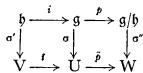
\includegraphics[keepaspectratio]{images/part001_4ab4ddcc.jpg}}

proves that \(\tilde{p}\) is zero on \(\sigma(\mathfrak{h})\) and hence on R. Let \(\psi\) be the canonical homomorphism of U onto U/R. There exists a homomorphism \(\phi\) of U/R

\pandocbounded{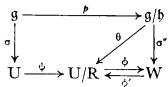
\includegraphics[keepaspectratio]{images/part001_c6a5c19d.jpg}}

into W such that \(\tilde{p} = \phi \circ \psi\) . The mapping \(\psi \circ \sigma\) of \(g\) into U/R is an \(\alpha\) -mapping and is zero on \(h\) and hence defines an \(\alpha\) -mapping \(\theta\) of \(g / h\) into U/R such that \(\theta \circ p = \psi \circ \sigma\) . Then \(\phi \circ \theta \circ p = \phi \circ \psi \circ \sigma = \sigma'' \circ p\) . Hence \(\phi \circ \theta = \sigma''\) . There exists (no. 1, Proposition 1) one and only one homomorphism \(\phi'\) of W into U/R mapping 1 to 1 and such that \(\theta = \phi' \circ \sigma''\) . Then \(\phi' \circ \phi \circ \theta = \phi' \circ \sigma'' = \theta\) and \(\phi \circ \phi' \circ \sigma'' = \phi \circ \theta = \sigma''\) and hence \(\phi' \circ \phi\) and \(\phi \circ \phi'\) are the identity mappings of U/R and W respectively. This completes the proof.

U/R is identified with W under the isomorphism \(\phi\) . Then the canonical mapping \(\sigma''\) of \(g/h\) into W is identified with \(\theta\) , that is with the mapping of \(g/h\) into U/R derived from \(\sigma\) by taking quotients.

\subsection{ENVELOPING ALGEBRA OF THE OPPOSITE LIE ALGEBRA}

Let \(g\) be a Lie algebra over \(K\) , \(g^0\) the opposite Lie algebra and \(\sigma\) and \(\sigma_0\) the canonical mappings of \(g\) and \(g^0\) into their enveloping algebras \(U\) and \(V\) . Then \(\sigma\) is an \(\alpha\) -mapping of \(g^0\) into the associative algebra \(U^0\) opposite to the associative algebra \(U\) . Hence there exists one and only one homomorphism \(\phi\) of \(V\) into \(U^0\) mapping 1 to 1 and such that \(\sigma = \phi \circ \sigma_0\) .

PROPOSITION 4. The homomorphism \(\phi\) is an isomorphism of \(V\) onto \(U^0\) .

There exists a homomorphism \(\phi'\) of U into \(V^0\) mapping 1 to 1 and such that \(\sigma_0 = \phi' \circ \sigma\) . \(\phi'\) can be considered as a homomorphism of \(U^0\) into V. Then \(\sigma_0 = \phi' \circ \phi \circ \sigma_0\) and \(\sigma = \phi \circ \phi' \circ \sigma\) and hence \(\phi' \circ \phi\) and \(\phi \circ \phi'\) are the identity mappings of V and U. Hence the proposition.

V is identified with \(U^{0}\) under the isomorphism \(\phi\) . Then \(\sigma_{0}\) is identified with \(\sigma\) .

With this identification, the isomorphism \(\theta: x \mapsto -x\) of \(\mathfrak{g}\) onto \(\mathfrak{g}^0\) defines an isomorphism \(\tilde{\theta}\) of U onto V = U \(^0\) . This isomorphism can be considered as an antiautomorphism of U. It is called the principal antiautomorphism of U. If \(x_{1}, \ldots, x_{n}\) are in \(\mathfrak{g}\) , then:

\[
\begin{array}{r l} \tilde {\theta} (\sigma (x _ {1}) \dots \sigma (x _ {n})) & = \tilde {\theta} (\sigma (x _ {n})) \dots \tilde {\theta} (\sigma (x _ {1})) = (- \sigma (x _ {n})) \dots (- \sigma (x _ {1})) \\ & = (- 1) ^ {n} \sigma (x _ {n}) \dots \sigma (x _ {1}). \end{array}\tag{2}
\]

\subsection{SYMMETRIC ALGEBRA OF A MODULE}

Let V be a K-module. V can be considered in a unique way as a commutative Lie algebra. The enveloping algebra of V can then be obtained as follows: let T be the tensor algebra of V; let I be the two-sided ideal of T generated by the tensors \(x \otimes y - y \otimes x\) ( \(x \in V, y \in V\) ); then form the algebra S = T/I.

Recalling (Algebra, Chapter III, § 6) that S is called the symmetric algebra of V, we summarize briefly the properties needed in this chapter, the proofs of which are immediate. Let \(T^{n}\) be the set of homogeneous tensors of order n in T. Then \(\mathrm{I} = (\mathrm{I} \cap \mathrm{T}^{2}) + (\mathrm{I} \cap \mathrm{T}^{3}) + \cdots\) and hence S is the direct sum of the canonical images \(S^{n}\) of the \(T^{n}\) . The elements of \(S^{n}\) are called homogeneous of degree n.~\(S^{0} = K.1\) , \(S^{1}\) is identified with V and \(S^{n}S^{p} \subset S^{n+p}\) . The algebra S is generated by 1 and \(S^{1} = V\) . Clearly any two elements of \(S^{1}\) are permutable and hence S is commutative. If V is a free K-module with basis \((x_{\lambda})_{\lambda \in \Lambda}\) , the canonical homomorphism f of the polynomial algebra \(K[X_{\lambda}]_{\lambda \in \Lambda}\) onto S which maps 1 to 1 and \(X_{\lambda}\) to \(x_{\lambda}\) for all \(\lambda \in \Lambda\) is an isomorphism: for by the universal property of S (no. 1, Proposition 1) there exists a homomorphism g of S into \(K[X_{\lambda}]_{\lambda \in \Lambda}\) which maps 1 to 1 and \(x_{\lambda}\) to \(X_{\lambda}\) for all \(\lambda \in \Lambda\) and f and g are inverse homomorphisms of one another.

Let \(S'^{n} \subset T^n\) be the set of homogeneous symmetric tensors of order \(n\) (Algebra, Chapter III, § 5, no. 1, Definition 2). If \(K\) is a field of characteristic 0, \(S'^{n}\) and \(I \cap T^n\) are supplementary in \(T^n\) . For let \((x_{\lambda})_{\lambda \in \Lambda}\) be a basis of \(V\) . We give \(\Lambda\) a total ordering (Set Theory, Chapter III, § 2, no. 3, Theorem 1). Let \(\Lambda_n\) be the set of increasing sequences of \(n\) elements of \(\Lambda\) . For \(M = (\lambda_1, \ldots, \lambda_n) \in \Lambda_n\) , let

\[
y _ {\mathrm{M}} = \frac {1}{n !} \sum_ {\sigma \in \mathfrak {S} _ {n}} x _ {\lambda_ {\sigma (1)}} \otimes \dots \otimes x _ {\lambda_ {\sigma (n)}}.
\]

The \(y_{\mathbf{M}}\) for \(\mathbf{M} \in \Lambda_n\) form a system of generators of the vector K-space \(\mathbf{S}'^n\) . Now their canonical images in \(\mathbf{S}^n\) constitute, by the above paragraph, a basis of \(\mathbf{S}^n\) . Hence \((y_{\mathbf{M}})_{\mathbf{M} \in \Lambda_n}\) is a basis of a supplementary subspace of \(\mathbf{I} \cap \mathbf{T}^n\) in \(\mathbf{T}^n\) (Algebra, Chapter II, § 1, no. 6, Proposition 4), which establishes our assertion.

Thus, when K is a field of characteristic 0, the restriction to \(S'^{n}\) of the canonical mapping \(T^{n} \rightarrow S^{n}\) is an isomorphism of the space \(S'^{n}\) onto the space \(S^{n}\) and therefore has an inverse isomorphism. The inverse isomorphisms thus obtained for each n define a canonical isomorphism of the space S onto the space \(S' = \sum_{n \geqslant 0} S'^{n}\) of symmetric tensors.

\subsection{FILTRATION OF THE ENVELOPING ALGEBRA}

Let g be a Lie algebra over K and T the tensor algebra of the K-module g. Let \(T^{n}\) be the submodule of T consisting of the homogeneous tensors of order n

and \(\mathrm{T_n} = \sum_{i\leqslant n}\mathrm{T^i}\) . Then \(\mathrm{T_n}\subset \mathrm{T}_{n + 1},\mathrm{T_0} = \mathrm{K}.1,\mathrm{T}_{-1} = \{0\}\) and \(\mathrm{T_nT_p}\subset \mathrm{T}_{n + p}\) . Let \(\mathbf{U}_n\) be the canonical image of \(\mathbf{T}_n\) in the enveloping algebra U of g. Then \(\mathrm{U_n}\subset \mathrm{U}_{n + 1},\mathrm{U_0} = \mathrm{K}.1,\mathrm{U}_{-1} = \{0\}\) and \(\mathrm{U_nU_p}\subset \mathrm{U}_{n + p}\) ; hence U can be described as an algebra filtered by the \(\mathbf{U}_n\) (Commutative Algebra, Chapter III, §2, no. I); the elements of \(\mathrm{U_n}\) will be said to be of filtration \(\leqslant n\) .

Let \(G^n\) be the K-module \(U_n / U_{n-1}\) and let G be the K-module the direct sum of the \(G^n\) . Multiplication on U defines, on taking quotients, a bilinear mapping of \(G^n \times G^m\) into \(G^{n+m}\) and hence a bilinear mapping of \(G \times G\) into G, which is associative. Thus G is given an associative K-algebra structure. Then \(G^n G^m \subset G^{n+m}\) . The elements of \(G^n\) are said to be of degree n.~The graded algebra thus obtained is just the graded algebra associated with the filtered algebra U (Commutative Algebra, Chapter III, § 2, no. 3).

Let \(\phi_{n}\) be the composition of the canonical K-linear mappings

\[
\mathrm{T} ^ {n} \rightarrow \mathrm{U} _ {n} \rightarrow \mathrm{G} ^ {n}.
\]

As \(\mathbf{T}^n\) is supplementary to \(\mathbf{T}_{n - 1}\) in \(\mathbf{T}_n\) , \(\phi_n\) is surjective. The \(\phi_n\) define a K-linear mapping \(\phi\) of \(\sum_{n}\mathbf{T}^{n} = \mathbf{T}\) onto \(\sum_{n}\mathbf{G}^{n} = \mathbf{G}\) .

PROPOSITION 5. The mapping \(\phi\) of T onto G is an algebra homomorphism mapping 1 to 1 and is zero on the two-sided ideal generated by the tensors \(x \otimes y - y \otimes x\) ( \(x \in \mathfrak{g}, y \in \mathfrak{g}\) ).

If \(t \in \mathbf{T}^n\) and \(t' \in \mathbf{T}^p\) , then \(\phi(t)\phi(t') = \phi(tt')\) by definition of the multiplication on \(\mathbf{G}\) . Hence \(\phi\) is an algebra homomorphism and clearly \(\phi(1) = 1\) . If \(x, y\) are in \(\mathfrak{g}\) , then \(x \otimes y - y \otimes x \in \mathbf{T}^2\) and the canonical image of this element in \(\mathrm{U}_2\) is equal to that of \([x, y]\) and therefore belongs to \(\mathrm{U}_1\) . Hence \(\phi(x \otimes y - y \otimes x) = 0\) , which proves the proposition.

Let S be the symmetric algebra of the K-module g and \(\tau\) the canonical homomorphism of T onto S. Proposition 5 proves that there exists a unique homomorphism \(\omega\) , called canonical, of the algebra S onto the algebra G, mapping 1 to 1, such that \(\phi = \omega \circ \tau\) . We have \(\omega(\mathrm{S}^{n}) = \phi(\mathrm{T}^{n}) = \mathrm{G}^{n}\) . Let \(\tau_{n}\) be the restriction of \(\tau\) to \(T^{n}\) , \(\omega_{n}\) the restriction of \(\omega\) to \(S^{n}\) , \(\psi_{n}\) the canonical mapping of \(T^{n}\) into \(U_{n}\) and \(\theta_{n}\) the canonical mapping of \(U_{n}\) onto \(G^{n}\) . The definition of \(\omega_{n}\) proves that the following diagram is commutative:

\pandocbounded{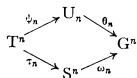
\includegraphics[keepaspectratio]{images/part001_82008693.jpg}}

PROPOSITION 6. If K is Noetherian and g is a finitely generated module, the ring U is right and left Noetherian.

S is a finitely generated algebra over K and hence a Noetherian ring (Commutative Algebra, Chapter III, § 2, no. 10, Corollary 3 to Theorem 2). Hence G, which is isomorphic to a quotient ring of S, is Noetherian. Hence U is right and left Noetherian (Commutative Algebra, Chapter III, § 2, no. 10, Remark 2).

COROLLARY. Suppose that K is a field and that g is finite-dimensional over K. Let \(I_{1}, \ldots, I_{m}\) be right (resp. left) ideals of finite codimension in U. Then the product ideal \(I_{1}I_{2}\ldots I_{m}\) is of finite codimension.

By induction on m it suffices to consider the case of, for example, two right ideals. The right U-module \(I_{1}\) is generated by a finite number of elements \(u_{1},\ldots,u_{p}\) (Proposition 6). Let \(v_{1},\ldots,v_{q}\) be elements of U whose classes modulo \(I_{2}\) generate the vector space \(U/I_{2}\) . Then the canonical images in \(I_{1}/I_{1}I_{2}\) of the \(u_{i}v_{j}\) generate the vector space \(I_{1}/I_{1}I_{2}\) , which is therefore finite-dimensional. Hence \(\dim_{\mathbb{K}}(\mathrm{U}/\mathrm{I}_{1}\mathrm{I}_{2})=\dim_{\mathbb{K}}(\mathrm{U}/\mathrm{I}_{1})+\dim_{\mathbb{K}}(\mathrm{I}_{1}/\mathrm{I}_{1}\mathrm{I}_{2})<+\infty\) .

Remark. Let \(g'\) be another Lie algebra over the ring K, \(U'\) its enveloping algebra, \(U_n'\) the set of elements of \(U'\) of filtration \(\leqslant n\) and \(U^n\) (resp. \(U'^n\) ) the set of canonical images in U (resp. \(U'\) ) of the homogeneous symmetric tensors of g (resp. \(g'\) ) of order n.~Let \(\eta\) be a homomorphism of g into \(g'\) and let \(\tilde{\eta}\) be the corresponding homomorphism of U into \(U'\) . Then

\[
\tilde {\eta} (\mathrm{U} _ {n}) \subset \mathrm{U} _ {n} ^ {\prime}, \quad \tilde {\eta} (\mathrm{U} ^ {n}) \subset \mathrm{U} ^ {\prime n}.
\]

In particular, the principal antiautomorphism of U leaves \(U_{n}\) and \(U^{n}\) stable. The K-linear mapping of \(T^{n}\) onto itself which maps

\[
x _ {1} \otimes x _ {2} \otimes \dots \otimes x _ {n} \quad \text { to } \quad x _ {n} \otimes x _ {n - 1} \otimes \dots \otimes x _ {1}
\]

for all \(x_{1},\ldots,x_{n}\) in g is a symmetry operator and hence leaves fixed the homogeneous symmetric tensors of order n.~Hence the principal antiautomorphism of U induces on each \(U^{n}\) the homothety of ratio \((-1)^{n}\) .

\subsection{THE POINCARÉ-BIRKHOFF-WITT THEOREM}

THEOREM 1. Let \(\mathfrak{g}\) be a Lie K-algebra, \(U\) its enveloping algebra, G the graded algebra associated with the filtered algebra U and S the symmetric algebra of the K-module \(\mathfrak{g}\) . If \(\mathfrak{g}\) is a free K-module, the canonical homomorphism \(\omega: \mathrm{S} \to \mathrm{G}\) is an isomorphism.

Let \((x_{\lambda})_{\lambda \in \Lambda}\) be a basis of the K-module g; we give \(\Lambda\) a total ordering (Set Theory, Chapter III, § 2, no. 3, Theorem 1). Let P be the polynomial algebra \(\mathrm{K}[z_{\lambda}]_{\lambda \in \Lambda}\) in indeterminates \(z_{\lambda}\) in one-to-one correspondence with the \(x_{\lambda}\) . For every sequence \(\mathrm{M} = (\lambda_1, \lambda_2, \ldots, \lambda_n)\) of elements of \(\Lambda\) , let \(z_{\mathrm{M}}\) denote the monomial \(z_{\lambda_1}z_{\lambda_2}\ldots z_{\lambda_n}\) and \(x_{\mathrm{M}}\) the tensor \(x_{\lambda_1}\otimes x_{\lambda_2}\otimes \dots \otimes x_{\lambda_n}\) .

The \(z_{\mathbb{M}}\) , for \(\mathbf{M}\) increasing, form a basis of the K-module \(\mathbf{P}\) (we make the convention that \(\varnothing\) is an increasing sequence and that \(z_{\varnothing} = 1\) ). Let \(\mathbf{P}_p\) be the submodule of polynomials of degree \(\leqslant p\) . We shall first prove several lemmas. (To abbreviate, we write \(\lambda \leqslant M\) if \(\lambda \leqslant \mu\) for every index \(\mu\) of the sequence M.)

Lemma 1. For every integer \(p \geqslant 0\) , there exists a unique homomorphism \(f_p\) of the K-module \(\mathfrak{g} \otimes_{\mathbb{K}} \mathrm{P}_p\) into the K-module \(\mathrm{P}\) satisfying the following conditions:

\[
\left(\mathrm{A} _ {p}\right) \quad f _ {p} \left(x _ {\lambda} \otimes z _ {\mathrm{M}}\right) = z _ {\lambda} z _ {\mathrm{M}} \quad \text {   for   } \lambda \leqslant \mathrm{M}, z _ {\mathrm{M}} \in \mathrm{P} _ {p};
\]

\[
\left(\mathrm{B} _ {p}\right) \quad f _ {p} \left(x _ {\lambda} \otimes z _ {\mathrm{M}}\right) - z _ {\lambda} z _ {\mathrm{M}} \in \mathrm{P} _ {q} \quad for \quad z _ {\mathrm{M}} \in \mathrm{P} _ {q}, q \leqslant p;
\]

\[
\left(\mathrm{C} _ {p}\right) \quad f _ {p} \left(x _ {\lambda} \otimes f _ {p} \left(x _ {\mu} \otimes z _ {\mathrm{N}}\right)\right) = f _ {p} \left(x _ {\mu} \otimes f _ {p} \left(x _ {\lambda} \otimes z _ {\mathrm{N}}\right)\right) + f _ {p} \left(\left[ x _ {\lambda}, x _ {\mu} \right] \otimes z _ {\mathrm{N}}\right)
\]

for \(z_{\mathbf{N}} \in \mathbf{P}_{p-1}\) . (The terms appearing in \((\mathbf{C}_p)\) are meaningful by \((\mathbf{B}_p)\) .)

Moreover, the restriction of \(f_{p}\) to \(\mathfrak{g} \otimes \mathrm{P}_{p-1}\) coincides with \(f_{p-1}\) .

The last assertion follows from the others since the restriction of \(f_{p}\) to \(\mathfrak{g} \otimes_{\mathbb{K}} \mathrm{P}_{p-1}\) satisfies conditions \((\mathrm{A}_{p-1})\) , \((\mathrm{B}_{p-1})\) and \((\mathrm{C}_{p-1})\) . We shall prove the existence and uniqueness of \(f_{p}\) by induction on \(p\) . For \(p = 0\) , condition \((\mathrm{A}_0)\) gives \(f_0(x_\lambda \otimes 1) = z_\lambda\) and conditions \((\mathrm{B}_0)\) and \((\mathrm{C}_0)\) are then obviously satisfied. Suppose now that the existence and uniqueness of \(f_{p-1}\) are proved. We show that \(f_{p-1}\) admits a unique extension \(f_{p}\) to \(\mathfrak{g} \otimes_{\mathbb{K}} \mathrm{P}_{p}\) satisfying conditions \((\mathrm{A}_{p})\) , \((\mathrm{B}_{p})\) and \((\mathrm{C}_{p})\) .

We must define \(f_{p}(x_{\lambda} \otimes z_{\mathbb{M}})\) for an increasing sequence M of p elements.

If \(\lambda \leqslant M\) , the value is given by condition \((A_p)\) . Otherwise, \(M\) can be written uniquely in the form \((\mu, N)\) , where \(\mu < \lambda\) , \(\mu \leqslant N\) . Then

\[
z _ {\mathrm{M}} = z _ {\mu} z _ {\mathrm{N}} = f _ {p - 1} (x _ {\mu} \otimes z _ {\mathrm{N}})
\]

by \((\mathrm{A}_{p - 1})\) , so that the left hand side of \((\mathrm{C}_p)\) is \(f_{p}(x_{\lambda}\otimes z_{\mathbb{M}})\) . Now the right hand side of \((\mathrm{C}_p)\) is already defined: for \((\mathrm{B}_{p - 1})\) allows us to write:

\[
f _ {p} (x _ {\lambda} \otimes z _ {\mathrm{N}}) = f _ {p - 1} (x _ {\lambda} \otimes z _ {\mathrm{N}}) = z _ {\lambda} z _ {\mathrm{N}} + w
\]

where \(w \in \mathbf{P}_{p-1}\) ; hence the right hand side of \((\mathbf{C}_p)\) becomes:

\[
z _ {\lambda} z _ {\mu} z _ {N} + f _ {p - 1} (x _ {\mu} \otimes w) + f _ {p - 1} ([ x _ {\lambda}, x _ {\mu} ] \otimes z _ {N}).
\]

Thus \(f_{p}\) is defined uniquely and obviously satisfies conditions \((\mathbf{A}_{p})\) and \((\mathbf{B}_{p})\) . Condition \((\mathbf{C}_{p})\) is satisfied if \(\mu < \lambda\) , \(\mu \leqslant N\) . As \([x_{\mu}, x_{\lambda}] = -[x_{\lambda}, x_{\mu}]\) , condition \((\mathbf{C}_{p})\) is also satisfied for \(\lambda < \mu\) , \(\lambda \leqslant N\) . As \((\mathbf{C}_{p})\) is trivially satisfied for \(\lambda = \mu\) , \((\mathbf{C}_{p})\) is therefore satisfied if \(\lambda \leqslant N\) or \(\mu \leqslant N\) . If none of these inequalities holds, \(N = (\nu, Q)\) , where \(\nu \leqslant Q\) , \(\nu < \lambda\) , \(\nu < \mu\) . Writing henceforth to abbreviate \(f_{p}(x \otimes z) = xz\) for \(x \in g\) and \(z \in P_{p}\) , we have by the induction hypothesis:

\[
x _ {\mu} z _ {N} = x _ {\mu} (x _ {\nu} z _ {Q}) = x _ {\nu} (x _ {\mu} z _ {Q}) + [ x _ {\mu}, x _ {\nu} ] z _ {Q}.
\]

Now \(x_{\mu}z_{\mathbf{Q}}\) is of the form \(z_{\mu}z_{\mathbf{Q}} + w\) , where \(w\in \mathrm{P}_{p - 2}\) . (C \(_{p}\) ) can be applied to \(x_{\lambda}(x_{\nu}(z_{\mu}z_{\mathbf{Q}}))\) , since \(\nu \leqslant Q\) and \(\nu < \mu\) , and to \(x_{\lambda}(x_{\nu}w)\) by the induction hypothesis, and hence to \(x_{\lambda}(x_{\nu}(x_{\mu}z_{\mathbf{Q}}))\) . Hence:

\[
\begin{array}{r l} x _ {\lambda} (x _ {\mu} z _ {N}) = x _ {\nu} (x _ {\lambda} (x _ {\mu} z _ {\mathbb {Q}})) & + [ x _ {\lambda}, x _ {\nu} ] (x _ {\mu} z _ {\mathbb {Q}}) + [ x _ {\mu}, x _ {\nu} ] (x _ {\lambda} z _ {\mathbb {Q}}) \\ & + [ x _ {\lambda}, [ x _ {\mu}, x _ {\nu} ] ] z _ {\mathbb {Q}}. \end{array}
\]

Exchanging \(\lambda\) and \(\mu\) and subtracting:

\[
\begin{array}{r l} {x _ {\lambda} (x _ {\mu} z _ {N}) - x _ {\mu} (x _ {\lambda} z _ {N})} & {= x _ {\nu} (x _ {\lambda} (x _ {\mu} z _ {Q}) - x _ {\mu} (x _ {\lambda} z _ {Q}))} \\ & {\quad + [ x _ {\lambda}, [ x _ {\mu}, x _ {\nu} ] ] z _ {Q} - [ x _ {\mu}, [ x _ {\lambda}, x _ {\nu} ] ] z _ {Q}} \\ & {= x _ {\nu} ([ x _ {\lambda}, x _ {\mu} ] z _ {Q}) + [ x _ {\lambda}, [ x _ {\mu}, x _ {\nu} ] ] z _ {Q} + [ x _ {\mu}, [ x _ {\nu}, x _ {\lambda} ] ] z _ {Q}} \\ & {= [ x _ {\lambda}, x _ {\mu} ] (x _ {\nu} z _ {Q}) + ([ x _ {\nu}, [ x _ {\lambda}, x _ {\mu} ] ]} \\ & {\quad + [ x _ {\lambda}, [ x _ {\mu}, x _ {\nu} ] ] + [ x _ {\mu}, [ x _ {\nu}, x _ {\lambda} ] ]) z _ {Q}} \end{array}
\]

and hence by the Jacobi identity

\[
x _ {\lambda} (x _ {\mu} z _ {N}) - x _ {\mu} (x _ {\lambda} z _ {N}) = [ x _ {\lambda}, x _ {\mu} ] z _ {N}
\]

which completes the proof of Lemma 1.

Lemma 2. There exists an \(\alpha\) -mapping \(\sigma\) of \(\mathfrak{g}\) into \(\mathcal{L}_{\mathbf{K}}(\mathbf{P})\) such that:

\begin{enumerate}
\def\labelenumi{(\arabic{enumi})}
\item
  \(\sigma(x_{\lambda})z_{\mathbf{M}} = z_{\lambda}z_{\mathbf{M}}\) for \(\lambda \leqslant \mathbf{M}\) ;
\item
  \(\sigma(x_{\lambda})z_{\mathbf{M}} \equiv z_{\lambda}z_{\mathbf{M}} (\mathrm{mod.~P}_{p})\) if \(\mathbf{M}\) has \(p\) elements.
\end{enumerate}

By Lemma 1 there exists a homomorphism \(f\) of the K-module \(\mathfrak{g} \otimes_{\mathbb{K}} \mathrm{P}_p\) into P satisfying, for all \(p\) , conditions \((\mathrm{A}_p), (\mathrm{B}_p), (\mathrm{C}_p)\) (where \(f_p\) is replaced by \(f\) ). This homomorphism defines a homomorphism \(\sigma\) of the K-module \(\mathfrak{g}\) into the K-module \(\mathcal{L}_{\mathbb{K}}(\mathrm{P})\) and \(\sigma\) is an \(\alpha\) -mapping because of condition \((\mathrm{C}_p)\) . Finally, \(\sigma\) satisfies properties (1) and (2) of the lemma because of conditions \((\mathrm{A}_p)\) and \((\mathrm{B}_p)\) .

Lemma 3. Let \(t\) be a tensor in \(\mathrm{T}_n \cap \mathrm{J}\) . The homogeneous component \(t_n\) of \(t\) of order \(n\) is in the kernel I of the canonical homomorphism \(\mathrm{T} \to \mathrm{S}\) .

We write \(t_n\) in the form \(\sum_{i=1}^{r} x_{\mathrm{M}_i}\) , where the \(\mathrm{M}_i\) are sequences of \(n\) elements of \(\Lambda\) . The mapping \(\sigma\) extends to a homomorphism of the algebra \(T\) into the algebra \(\mathcal{L}_K(P)\) (which we shall also denote by \(\sigma\) ), which is zero on \(J\) . By Lemma 2, \(\sigma(t)\) . 1 is a polynomial whose terms of highest degree are \(\sum_{i=1}^{r} z_{\mathrm{M}_i}\) . As \(t \in J\) , \(\sigma(t) = 0\) and hence \(\sum_{i=1}^{r} z_{\mathrm{M}_i} = 0\) in \(P\) . Now \(P\) is canonically identified with \(S\) , since \(g\) has basis \((x_\lambda)\) . Hence the canonical image of \(t_n\) in \(S\) is zero, that is \(t_n \in I\) .

We can now prove Theorem 1. It is necessary to prove that the canonical homomorphism of S onto G is injective. In other words, if \(t \in \mathrm{T}^n\) and \(\psi\) denotes the canonical homomorphism of T onto U, it is necessary to show that the condition \(\psi(t) \in \mathrm{U}_{n-1}\) implies \(t \in I\) . Now \(\psi(t) \in \mathrm{U}_{n-1}\) means that there exists a tensor \(t' \in \mathrm{T}_{n-1}\) such that \(t - t' \in J\) . The tensor \(t - t'\) admits \(t\) as homogeneous component of order \(n\) and hence \(t \in I\) by Lemma 3.

COROLLARY 1. Suppose that \(\mathfrak{g}\) is a free K-module. Let W be a sub-K-module of \(\mathbf{T}^n\) .

If, in the notation of diagram (3), the restriction of \(\tau_{n}\) to W is an isomorphism of W onto \(\mathbf{S}^n\) , then the restriction of \(\psi_{n}\) to W is an isomorphism of W onto a supplement of \(\mathbf{U}_{n-1}\) in \(\mathbf{U}_n\) .

The restriction to W of \(\omega_{n} \circ \tau_{n}\) is a bijection of W onto \(G^{n}\) ; so is the restriction \(\theta_{n} \circ \psi_{n}\) to W. Hence the corollary.

COROLLARY 2. If \(\mathfrak{g}\) is a free K-module, the canonical mapping of \(\mathfrak{g}\) into its enveloping algebra is injective.

This follows from Corollary 1 taking \(\mathbf{W} = \mathbf{T}^1\)

When g is a free K-module (in particular when K is a field), g is identified with a submodule of U under the canonical mapping of g into U. This convention is adopted from the following corollary onwards.

COROLLARY 3. If \(\mathfrak{g}\) admits a totally ordered basis \((x_{\lambda})_{\lambda \in \Lambda}\) , the elements \(x_{\lambda_1}x_{\lambda_2}\ldots x_{\lambda_n}\) of the enveloping algebra \(\mathbf{U}\) , where \((\lambda_1,\dots ,\lambda_n)\) is an arbitrary increasing finite sequence of elements of \(\Lambda\) , form a basis of the K-module \(\mathbf{U}\) .

Let \(\Lambda_{n}\) be the set of increasing sequences of \(n\) elements of \(\Lambda\) . For \(\mathrm{M} = (\lambda_1, \ldots, \lambda_n) \in \Lambda_n\) , let \(y_{\mathrm{M}} = x_{\lambda_1} \otimes x_{\lambda_2} \otimes \dots \otimes x_{\lambda_n}\) . Let \(\mathrm{W}\) be the submodule of \(\mathrm{T}^n\) with basis \((y_{\mathrm{M}})_{\mathrm{M} \in \Lambda_n}\) . Corollary 1 shows that the restriction of \(\psi_n\) to \(\mathrm{W}\) is an isomorphism of \(\mathrm{W}\) onto a supplement of \(\mathrm{U}_{n-1}\) in \(\mathrm{U}_n\) . But

\[
\psi_ {n} (y _ {\mathrm{M}}) = x _ {\lambda_ {1}} x _ {\lambda_ {2}} \dots x _ {\lambda_ {n}},
\]

whence the corollary.

COROLLARY 4. Let \(S'^{n} \subset T^n\) be the set of homogeneous symmetric tensors of order \(n\) . Suppose that \(K\) is a field of characteristic 0. Then the composite mapping of the canonical mappings

\[
\mathrm{S} ^ {n} \rightarrow \mathrm{S} ^ {\prime n} \rightarrow \mathrm{U} _ {n}
\]

is an isomorphism of the vector space \(\mathbf{S}^n\) onto a supplement of \(\mathbf{U}_{n-1}\) in \(\mathbf{U}_n\) .

This follows from Corollary 1 taking \(W = S'^n\) .

Suppose henceforth that \(\mathbf{K}\) is a field of characteristic 0. Let \(\eta_{n}\) be the mapping of \(S^n\) into \(U_n\) just defined. Let \(U^n = \eta_n(S^n)\) . The vector space \(U\) is the direct sum of the \(U^n\) . The \(\eta_{n}\) define an isomorphism \(\eta\) of the vector space \(S = \sum_{n} S^n\) onto the vector space \(U = \sum_{n} U^n\) , called the canonical isomorphism of \(S\) onto \(U\) ; this is not an algebra isomorphism. We have the commutative diagram:

\pandocbounded{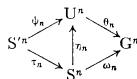
\includegraphics[keepaspectratio]{images/part001_756df219.jpg}}

where each arrow represents a vector space isomorphism. If \(x_{1}, x_{2}, \ldots, x_{n}\) are in \(g\) , \(\eta_{n}\) maps the product \(x_{1}x_{2}\ldots x_{n}\) , calculated in S, to the element

\[
\frac {1}{n !} \sum_ {\sigma \in \mathfrak {S} _ {n}} x _ {\sigma (1)} x _ {\sigma (2)} \dots x _ {\sigma (n)}
\]

calculated in U.

COROLLARY 5. Let \(\mathfrak{h}\) be a subalgebra of the Lie algebra \(\mathfrak{g}\) and \(\mathrm{U}'\) its enveloping algebra. Suppose that the K-modules \(\mathfrak{h}\) and \(\mathfrak{g} / \mathfrak{h}\) are free (for example if \(\mathrm{K}\) is a field). Let \((x_{\alpha})_{\alpha \in \mathbb{L}}\) be a basis of \(\mathfrak{h}\) and \((y_{\beta})_{\beta \in \mathbb{M}}\) a family of elements of \(\mathfrak{g}\) whose canonical images in \(\mathfrak{g} / \mathfrak{h}\) form a basis of \(\mathfrak{g} / \mathfrak{h}\) .

\begin{enumerate}
\def\labelenumi{(\alph{enumi})}
\item
  The canonical homomorphism of \(\mathbf{U}'\) into \(\mathbf{U}\) is injective.
\item
  If \(\mathbf{M}\) is totally ordered, the elements \(y_{\beta_1} \ldots y_{\beta_q}\) , where \(\beta_1 \leqslant \cdots \leqslant \beta_q\) , form a basis of \(\mathbf{U}\) considered as a left or right module over \(\mathbf{U}'\) .
\end{enumerate}

We give \(L \cup M\) a total ordering such that every element of L is less than every element of M. The elements \(x_{\alpha_{1}}x_{\alpha_{2}}\ldots x_{\alpha_{p}}\) calculated in \(U'\) (where \(\alpha_{1} \leqslant \cdots \leqslant \alpha_{p}\) ) form a basis of \(U'\) (Corollary 3). The elements

\[
x _ {\alpha_ {1}} \dots x _ {\alpha_ {p}} y _ {\beta_ {1}} \dots y _ {\beta_ {q}}
\]

calculated in U (where \(\alpha_{1} \leqslant \cdots \leqslant \alpha_{p} \leqslant \beta_{1} \leqslant \cdots \leqslant \beta_{q}\) ) similarly form a basis of U. Hence the canonical homomorphism of U' into U maps the elements of a basis of U' to linearly independent elements of U and is therefore injective. It is moreover seen that the \(y_{\beta_1} \ldots y_{\beta_q}\) (where \(\beta_{1} \leqslant \cdots \leqslant \beta_{q}\) ) form a basis of U considered as a left U'-module. Ordering L ∪ M so that every element of M is less than every element of L, it is similarly seen that the \(y_{\beta_1} \ldots y_{\beta_q}\) (where \(\beta_{1} \leqslant \cdots \leqslant \beta_{q}\) ) form a basis of U considered as a right U'-module.

Under the conditions of Corollary 5, U' is identified with the subalgebra of U generated by h by means of the canonical homomorphism of U' into U.

COROLLARY 6. Suppose that the K-module g is the direct sum of subalgebras \(g_{1}, g_{2}, \ldots, g_{n}\) and that each \(g_{i}\) is a free K-module. Let \(U_{i}\) be the enveloping algebra of \(g_{i}\) ( \(1 \leqslant i \leqslant n\) ). Let \(\phi\) be the K-linear mapping of the K-module \(U_{1} \otimes_{K} \cdots \otimes_{K} U_{n}\) into U defined by the multilinear mapping ( \(u_{1}, \ldots, u_{n}\) ) \(\mapsto u_{1} \ldots u_{n}\) of \(U_{1} \times \cdots \times U_{n}\) into U. Then \(\phi\) is a K-module isomorphism.

Let \((x_{\lambda}^{i})_{\lambda \in L_{i}}\) be a basis of \(g_{i}\) . We totally order \(L_{1} \cup \cdots \cup L_{n}\) so that every element of \(L_{i}\) exceeds every element of \(L_{j}\) for \(i \geqslant j\) . Then the elements:

\[
\left(x _ {\lambda_ {1}} ^ {1} x _ {\lambda_ {2}} ^ {1} \dots x _ {\lambda_ {p}} ^ {1}\right) \otimes \dots \otimes \left(x _ {\nu _ {1}} ^ {n} x _ {\nu _ {2}} ^ {n} \dots x _ {\nu _ {q}} ^ {n}\right),
\]

where \(\lambda_{1}\leqslant\lambda_{2}\leqslant\cdots\leqslant\lambda_{p}\leqslant\cdots\leqslant\nu_{1}\leqslant\nu_{2}\leqslant\cdots\leqslant\nu_{q}\) , constitute a basis of \(U_{1}\otimes_{K}\cdots\otimes_{K}U_{n}\) . They are mapped by \(\phi\) to the elements:

\[
x _ {\lambda_ {1}} ^ {1} x _ {\lambda_ {2}} ^ {1} \dots x _ {\lambda_ {p}} ^ {1} \dots x _ {\nu_ {1}} ^ {n} x _ {\nu_ {2}} ^ {n} \dots x _ {\nu_ {q}} ^ {n}
\]

which constitute a basis of U. Hence the corollary.

COROLLARY 7. If K is an integral domain and g is a free K-module, the algebra U has no divisors of zero.

G is isomorphic to a polynomial algebra over K (Theorem 1) and is therefore an integral domain (Algebra, Chapter IV, § 1, no. 4, Theorem 1). Hence the corollary (Commutative Algebra, Chapter III, § 2, no. 3, Proposition 1).

\subsection{EXTENSION OF DERIVATIONS}

Lemma 4. Let V be a K-module and T the tensor algebra of V. Let u be an endomorphism of V. There exists one and only one derivation of T which extends u. This derivation commutes with the symmetry operators on T.

Let \(F = V \times V \times \cdots \times V\) (n factors). The mapping

\[
\begin{array}{r l} (x _ {1}, \ldots , x _ {n}) & \mapsto u x _ {1} \otimes x _ {2} \otimes \dots \otimes x _ {n} \\ & \qquad + x _ {1} \otimes u x _ {2} \otimes \dots \otimes x _ {n} + \dots + x _ {1} \otimes x _ {2} \otimes \dots \otimes u x _ {n} \end{array}
\]

of F into \(\bigotimes^{n}\) V is multilinear. Hence there exists an endomorphism \(u_{n}\) of \(\bigotimes^{n}\) V such that:

\[
u _ {n} \left(x _ {1} \otimes \dots \otimes x _ {n}\right) = u x _ {1} \otimes \dots \otimes x _ {n} + \dots + x _ {1} \otimes \dots \otimes u x _ {n}
\]

for all \(x_1, \ldots, x_n\) in V. Then \(u_1 = u\) . Let \(v\) be the endomorphism of the K-module T which coincides with \(u_n\) on each \(\mathrm{T}^n = \bigotimes^n \mathrm{V}\) and which is zero on \(\mathrm{T}^0 = \mathrm{K}. 1\) . We show that \(v\) is a derivation of T. If \(x_1, \ldots, x_n, y_1, \ldots, y_p\) are elements of V, then

\[
\begin{array}{l} v ((x _ {1} \otimes \dots \otimes x _ {n}) \otimes (y _ {1} \otimes \dots \otimes y _ {p})) \\ = \sum_ {i = 1} ^ {n} x _ {1} \otimes \dots \otimes x _ {i - 1} \otimes u x _ {i} \otimes x _ {i + 1} \otimes \dots \otimes x _ {n} \otimes y _ {1} \otimes \dots \otimes y _ {p} \\ \qquad + \sum_ {j = 1} ^ {p} x _ {1} \otimes \dots \otimes x _ {n} \otimes y _ {1} \otimes \dots \otimes y _ {j - 1} \otimes u y _ {j} \otimes y _ {j + 1} \otimes \dots \otimes y _ {p} \\ = v (x _ {1} \otimes \dots \otimes x _ {n}) \otimes (y _ {1} \otimes \dots \otimes y _ {p}) + (x _ {1} \otimes \dots \otimes x _ {n}) \otimes v (y _ {1} \otimes \dots \otimes y _ {p}). \end{array}
\]

By linearity it follows that \(v\) is a derivation. The uniqueness of \(v\) is obvious.

Finally, clearly \(u_{n}\) commutes with all the symmetry operators on \(\otimes V\) , whence the last assertion.

PROPOSITION 7. Let \(\mathfrak{g}\) be a Lie algebra, U its enveloping algebra, \(\sigma\) the canonical mapping of \(\mathfrak{g}\) into U and D a derivation of \(\mathfrak{g}\) .

\begin{enumerate}
\def\labelenumi{(\alph{enumi})}
\item
  There exists one and only one derivation \(\mathrm{D_U}\) of U such that \(\sigma \circ \mathrm{D} = \mathrm{D_U} \circ \sigma\) (that is such that \(\mathrm{D_U}\) extends D, when \(\mathfrak{g}\) can be identified with a submodule of U under \(\sigma\) ).
\item
  \(D_{U}\) leaves stable \(U_{n}\) and the set \(U^{n}\) of images in U of the homogeneous symmetric tensors of order n over g.
\item
  \(\mathbf{D}_{\mathbf{U}}\) commutes with the principal antiautomorphism of \(\mathbf{U}\) .
\item
  If \(\mathbf{D}\) is the inner derivation of \(\mathfrak{g}\) defined by an element \(x\) of \(\mathfrak{g}\) , \(\mathrm{D}_{\mathbf{U}}\) is the inner derivation of \(\mathbf{U}\) defined by \(\sigma(x)\) .
\end{enumerate}

Let \(D_T\) be the derivation of the tensor algebra \(T\) of \(g\) which extends \(D\) (Lemma 4). The two-sided ideal \(J\) of \(T\) generated by the

\[
x \otimes y - y \otimes x - [ x, y ]
\]

\((x,y \text{ in } \mathfrak{g})\) is stable under \(\mathrm{D}_{\mathrm{T}}\) . For:

\[
\begin{array}{r} \mathrm{D} _ {\mathrm{T}} (x \otimes y - y \otimes x - [ x, y ]) = \mathrm{D} x \otimes y - y \otimes \mathrm{D} x - [ \mathrm{D} x, y ] \\ + x \otimes \mathrm{D} y - \mathrm{D} y \otimes x - [ x, \mathrm{D} y ]. \end{array}
\]

On passing to the quotient, \(D_{T}\) defines a derivation \(D_{U}\) of U such that \(\sigma \circ D = D_{U} \circ \sigma\) . The uniqueness of \(D_{U}\) is immediate since 1 and \(\sigma(\mathfrak{g})\) generate the algebra U. Assertion (b) is obvious. Let A be the principal antiautomorphism of U. We now prove (c). If \(x_{1}, \ldots, x_{n}\) are in g, then

\[
\begin{array}{r l} \mathrm{D} _ {\mathrm{U}} \mathrm{A} (\sigma (x _ {1}) \dots \sigma (x _ {n})) & = \mathrm{D} _ {\mathrm{U}} ((- 1) ^ {n} \sigma (x _ {n}) \dots \sigma (x _ {1})) \\ & = (- 1) ^ {n} \sum_ {i = 1} ^ {n} \sigma (x _ {n}) \dots \mathrm{D} _ {\mathrm{U}} (\sigma (x _ {i})) \dots \sigma (x _ {1}) \\ & = (- 1) ^ {n} \sum_ {i = 1} ^ {n} \sigma (x _ {n}) \dots \sigma (\mathrm{D} x _ {i}) \dots \sigma (x _ {1}) \\ & = \mathrm{A} \bigg (\sum_ {i = 1} ^ {n} \sigma (x _ {1}) \dots \sigma (\mathrm{D} x _ {i}) \dots \sigma (x _ {n}) \bigg) \\ & = \mathrm{AD} _ {\mathrm{U}} (\sigma (x _ {1}) \dots \sigma (x _ {n})). \end{array}
\]

Finally, let \(x \in \mathfrak{g}\) . Let \(\Delta\) be the inner derivation \(y \mapsto \sigma(x)y - y\sigma(x)\) of U (Algebra, Chapter IV, § 4, no. 3, Example 2). Then, for \(x' \in \mathfrak{g}\) ,

\[
(\Delta \circ \sigma) (x ^ {\prime}) = \sigma (x) \sigma (x ^ {\prime}) - \sigma (x ^ {\prime}) \sigma (x) = \sigma ([ x, x ^ {\prime} ]) = (\sigma \circ \operatorname{ad} x) (x ^ {\prime}),
\]

whence \(\Delta \circ \sigma = \sigma \circ \operatorname{ad} x\) . This completes the proof.

Applying Proposition 7 to the case of a commutative Lie algebra, it is seen that every endomorphism u of a K-module can be extended uniquely to a derivation of the symmetric algebra of this module; this derivation is derived on passing to the quotient from the derivation of the tensor algebra which extends u.

We again take a Lie algebra g over K and let D be a derivation of g. We use the earlier notation T, S, U, G. Let \(D_{T}\) , \(D_{S}\) be the derivations of T, S which extend D and let \(D_{U}\) be the unique derivation of U such that \(\sigma \circ D = D_{U} \circ \sigma\) . Since \(D_{U}\) leaves the \(U_{n}\) stable, \(D_{U}\) defines on taking quotients a derivation \(D_{G}\) of G. Since \(D_{U}\) and \(D_{S}\) are derived from \(D_{T}\) when passing to quotients, the commutative diagram (3) proves that \(D_{G}\) can also be derived from \(D_{S}\) by the homomorphism \(\omega\) defined in no. 6. If further K is a field of characteristic 0, the isomorphisms of diagram (4) map one into another the restrictions of \(D_{T}\) , \(D_{S}\) , \(D_{U}\) , \(D_{G}\) to \(S^{n}\) , \(S^{n}\) , \(U^{n}\) , \(G^{n}\) . Hence the canonical isomorphism of S onto U maps \(D_{S}\) to \(D_{U}\) .

\subsection{EXTENSION OF THE BASE RING}

Let g be a Lie algebra over K, T its tensor algebra, J the two-sided ideal of T generated by the \(x \otimes y - y \otimes x - [x, y]\) (x, y in g) and U = T/J. Let \(K_{1}\) be a commutative ring with unit element and \(\sigma\) a homomorphism of K into \(K_{1}\) mapping 1 to 1. Then the tensor algebra of \(\mathfrak{g}_{(\mathbf{K}_{1})}\) is canonically identified with \(\mathrm{T}_{(\mathbf{K}_{1})}\) . Let \(J'\) be the two-sided ideal of \(\mathrm{T}_{(\mathbf{K}_{1})}\) generated by the

\[
x ^ {\prime} \otimes y ^ {\prime} - y ^ {\prime} \otimes x ^ {\prime} - [ x ^ {\prime}, y ^ {\prime} ]
\]

\((x', y' \text{ in } g_{(K_1)})\) . Clearly the canonical image of \(J_{(K_1)}\) in \(T_{(K_1)}\) is contained in \(J'\) . To see that it is equal to \(J'\) , it suffices to show that, if \(x'\) and \(y'\) denote two elements of \(g_{(K_1)}\) , \(x' \otimes y' - y' \otimes x' - [x', y']\) belongs to this image. Now

\[
x ^ {\prime} = \sum_ {i} x _ {i} \otimes \lambda_ {i}, y ^ {\prime} = \sum_ {j} y _ {j} \otimes \mu_ {j} (x _ {i}, y _ {j} \text {   in   } \mathfrak {g}, \lambda_ {i}, \mu_ {j} \text {   in   } \mathrm{K} _ {1});
\]

whence

\[
x ^ {\prime} \otimes y ^ {\prime} - y ^ {\prime} \otimes x ^ {\prime} - [ x ^ {\prime}, y ^ {\prime} ] = \sum_ {i, j} (x _ {i} \otimes y _ {j} - y _ {j} \otimes x _ {i} - [ x _ {i}, y _ {j} ]) \otimes \lambda_ {i} \mu_ {j}
\]

which proves our assertion. Then it can be seen that \(\mathrm{U}_{(\mathbf{K}_{1})} = (\mathrm{T}/\mathrm{J})_{(\mathbf{K}_{1})}\) is canonically identified with \(\mathrm{T}_{(\mathbf{K}_{1})}/\mathrm{J}'\) : the enveloping algebra of \(\mathfrak{g}_{(\mathbf{K}_{1})}\) is canonically identified with \(\mathrm{U}_{(\mathbf{K}_{1})}\) and the canonical mapping of \(\mathfrak{g}_{(\mathbf{K}_{1})}\) into its enveloping algebra is identified with \(\sigma \otimes 1\) (where \(\sigma\) denotes the canonical mapping of g into U).

\section{REPRESENTATIONS}

